\chapter{基于Top-K混洗差分隐私的联邦学习模型}
\label{ch4}
\section{引言}
上一章节中所提出的本地自适应差分隐私方案是通过在客户端将梯度上传至参数服务器前,对梯度添加自适应噪声实现全局模型的差分隐私。尽管方案采用了梯度自适应加躁和裁剪算法减少一定程度的模型精度损失,但Truex等人\upcite{ref49}指出的,一个复杂的本地隐私保护联邦学习系统将多个本地差分隐私的算法进行组合,会导致总体的隐私成本增长。如果每个本地用户都需要在训练过程中添加$O(1)$,中央服务器将各个数据聚合后,总体噪声的方差达到$O(n)$, 标准差达到$O(\sqrt{n})$。在本地设备的模型训练上采用差分隐私技术,对于聚合后的梯度平均估计误差能达到$O\left(\frac{\sqrt{d \log d}}{\epsilon \sqrt{m}}\right)$。使用联邦学习训练的联合模型需要客户在多次迭代中向中央服务器上传梯度更新。如果在迭代训练过程中的每一次迭代都应用本地差分隐私,隐私损耗就会成倍累积,从而导致聚合参数上的噪声溢出,影响全局模型的发布结果。在实际的联邦学习应用场景中,本地客户端的数量可能超过千万量级,中央服务器对所有本地上传的加躁梯度进行聚合时,可能因为噪声量的聚合而导致原有的梯度信息被累积的噪声淹没,从而大大降低模型的精度,也增加了通信开销。

在最近的研究工作中,Bittau等人提出了一个新的隐私保护框架(Encode-Shuffle-Analyze,ESA)。ESA框架包含n个编码器、一个洗牌器和一个分析器。
\begin{enumerate}
\item [(1)] 编码器$R: \mathcal{X} \rightarrow y^{m}$:编码器对用户的输入数据 $x_{i}$进行加密或者扰动,得到$y_{i, 1}, \ldots, y_{i, m} \in y$
\item [(2)] 洗牌器$S:\left(y^{m}\right)^{n} \rightarrow y^{m n}$:洗牌器可以看作是一个可信任的实体,独立于分析器,接收n个用户上传的加密数据,对上传的数据集合中的元素进行随机置换,得到无序集合再上传至分析器
\item [(3)] 分析器$A: y^{m n} \rightarrow \mathcal{Z}$:分析器将混洗器的所有输出信息作为输入,运行全局的聚合函数。
\end{enumerate}

ESA框架是一个针对n个客户和一个中央服务器的隐私保护框架,每个客户本地运行一个编码器,对于所要上传的数据进行加密处理,每个客户可以提交一条或多条消息。相比于客户端直接将消息上传至分析器,ESA通过在分析器和编码器增加洗牌器,将所有客户上传的加密数据集合中的向量元素进行拆分和随机置换,得到一个无序的消息集合(不包含任何标识信息),于是分析器没有能力获得客户端的IP地址、信息上传的时间戳和路由路径等用户隐私。

本文根据前人的研究思路,通过在联邦学习中应用ESA框架实现分布式的差分隐私,也叫做混洗差分隐私。本文在联邦学习模型中新增混洗器,混洗器通过对梯度进行动态采样和随机扰动。相比于在原有的EA框架中直接应用本地差分隐私,混洗差分隐私在模型可用性方面提高了$O(\sqrt{n})$ 倍,接近于中央差分隐私的水平。混洗差分隐私在模型准确率方面的增益来源于隐私放大效应,对本地设备的输出进行混洗后在差分隐私的中心视图中比没有混洗的输出提供更强的隐私效用,对于不受信任的中央服务器要达到相同的隐私保护水平,所需要添加的本地噪音更少。本方案通过采样和混洗达到双重的隐私放大,将$\left(\epsilon_{1}+\epsilon_{2}\right)$的本地隐私预算放大至$\epsilon-$中央差分隐私,降低了隐私成本。

此外,在联邦学习的应用场景中,有些本地用户所提供的连接可能为低带宽,巨大的模型参数量给通信网络带来了高负荷的运输负担,那么就需要对服务端和客户端之间的通信带宽进行限制。模型的通信开销受到模型参数大小、客户端数量、通信回合等影响。在全局聚合过程中由于不同的客户端训练和处理数据的速度不同,还可能带来额外的网络延迟。提高联邦学习通信效率的策略分为两种,其一,在联邦学习训练期间减少服务器和客户端之间的通信回合数;其二,在每一次服务器和客户端的通信过程中传输更少的参数。现有的研究包括使用静态抽样来选择一部分客户模型参与全局更新,或者对客户端上传的参数使用压缩算法来提高通信效率。基于具有较大绝对值的梯度可以为模型收敛做出更多贡献的事实,本文创造性地设计了客户端梯度的Top-K采样算法,采用指数机制的打分原理挑选出绝对值排名前k位的梯度元素,添加拉普拉斯扰动,实现二阶段的扰动,使本地训练所得的梯度满足$\left(\epsilon_{1}+\epsilon_{2}\right)$-差分隐私。该方案在相同的中央差分隐私预算下降低了通信成本,缓解了由维度系数增加而带来的隐私成本溢出和模型精度下降的问题。

% 综上所述,本文主要针对通信开销、隐私成本溢出等问题,对联邦学习隐私保护方案进行改进,创新点主要有三个方面:
% \begin{enumerate}
% \item [(1)] 根据指数机制,对本地客户端训练所得的梯度进行top-K采样和概率选择,保留对于模型收敛更重要的元素。对于top-K的梯度添加拉普拉斯扰动,使本地训练所得的梯度满足$\left(\epsilon_{1}+\epsilon_{2}\right)$-差分隐私
% \item [(2)] 在中央服务器和本地客户端之间新增混洗器,混洗器对梯度元素进行随机置换,得到无序的消息集合对
% \item [(3)] 通过
% \end{enumerate}

\section{模型设计}
在本文的方案中,假设敌手为为恶意的第三方服务器和诚实但好奇的中央服务器,中央服务器诚实的依据联邦学习的协议完成全局模型的训练,但是它持有用户所上传的梯度的信息,有可能损害用户的隐私数据。此外,我们假设中央服务器和第三方服务器之间不存在串通、混洗器和中央服务器之间不存在串通。

基于上述的威胁模型,隐私要求表述如下:
\begin{itemize}
  \item 用户的本地梯度的保密性:敌手如中央服务器服务器,可能通过用户上传的梯度信息和模型的全局参数恢复得到用户本地数据信息,比如数据标签和成员信息。为了实现用户数据的隐私性,每个本地梯度在被发送到服务器之前应该通过安全加密。
  \item 用户所选择的Top-K梯度索引信息的保密性:虽然用户上传的梯度值是添加噪声之后的,但是由于梯度的绝对值和其索引信息是一并发送给混洗器的,本方案需要约束中央服务器成功预测一个索引是否在用户本地向量上传的Top-k元素中。
  \item 用户的数据质量的保密性:在联邦学习中,不同的用户数据对于全局模型的训练影响不同,为了保证训练过程的公正,以及防止敌手获取用户的可靠性信息进行联合攻击,用户的数据质量也需要加密,防止任何第三方和中央服务器获取。
\end{itemize}

\subsection{模型概览}
\begin{figure}[!hbt]
\centering
	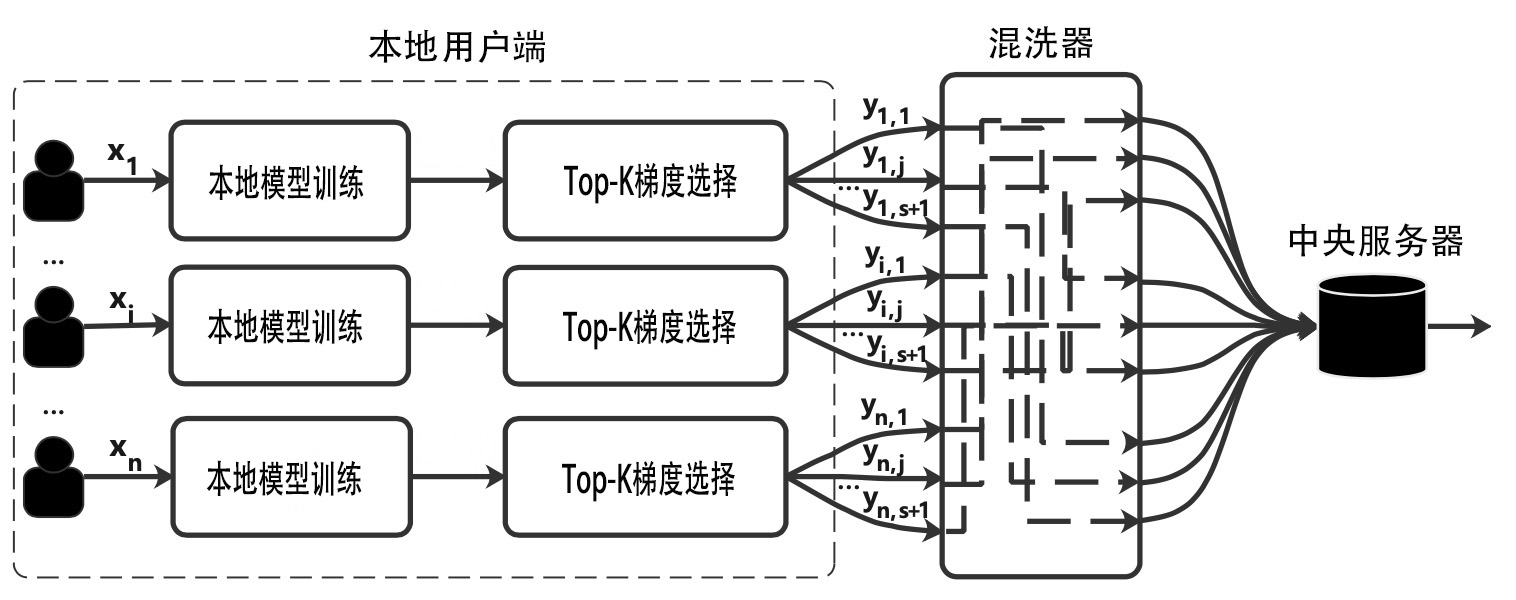
\includegraphics[scale=0.5]{fig2/C4/模型概况图}%联邦学习的系统架构
	\caption{基于top-K安全混洗的联邦学习框架}
	\label{fig:基于安全混洗和Top-K梯度选择算法的联邦学习模型框架}	
\end{figure}

如图\ref{fig:基于安全混洗和Top-K梯度选择算法的联邦学习模型框架}所示,基于top-K安全混洗的联邦学习框架主要由本地客户端、混洗器和中央服务器3部分组成:
\begin{itemize}
  \item 本地客户端:本地设备通过模型训练得到梯度向量$\mathbf{g}$,根据向量中每一元素的绝对值进行降序排序,以较大的概率选择为top-K元素的梯度值,在梯度上添加拉普拉斯噪声,再以较小的概率选择非top-K元素的梯度值
,得到满足$\left(\epsilon_{1}+\epsilon_{2}\right)-LDP$的索引列表和梯度元素列表。
  \item 混洗器:动态采样客户端的梯度,然后对梯度中的元素排列进行随机置换,通过双重隐私放大效应使得算法满足$(\epsilon, \delta)$-差分隐私,达到梯度匿名机制,最后将混洗后的结果发送至中央服务器。
  \item 中央服务器:一个诚实但好奇的第三方。服务器接受混洗器上传的梯度元素列表和索引列表进行加权聚合后更新全局模型。
\end{itemize}

假设现在有m个本地客户端,每个客户端表示为$i \in[m]$,其本地数据集为\\$\mathcal{D}_{i}=\left\{d_{i 1}, \ldots, d_{i r}\right\} \in \mathbb{S}^{r}$。$F_{i}(\theta)$表示在客户端$i$的本地数据集 $\mathcal{D}_{i}$上进行训练,对于模型梯度$\theta \in \mathbb{R}^{d}$进行衡量的损失函数,其中$F_{i}(\theta)=\frac{1}{r} \sum_{j=1}^{r} f\left(\theta ; d_{i j}\right)$,$f(\theta ; \cdot): \mathcal{C} \rightarrow \mathbb{R}$是凸函数。中央服务器的目标是找到一个最佳的模型参数向量$\theta^{*} \in \mathcal{C}$ 使得全局ERM最小:$\min _{\theta \in \mathcal{C}}\left(F(\theta)=\frac{1}{m} \sum_{i=1}^{m} F_{i}(\theta)\right)$,其中隐私性满足总体模型的隐私预算,也就是满足$(\epsilon, \delta)$-差分隐私。

在算法\ref{联邦学习中的安全混洗算法}中,首先每个客户端$i \in \mathcal{U}_{t}$从本地数据集中抽样$\mathcal{S}_{i t}$个样本训练模型,计算梯度$\nabla_{\theta_{t}} f\left(\theta_{t} ; d_{i j}\right)$,然后运行Top-K梯度选择算法对梯度进行采样扰动,得到满足$\left(\epsilon_{1}+\epsilon_{2}\right)-LDP$的梯度元素列表和索引列表$\left\langle index_{i,j}, y_{i,j}\right\rangle$。混洗器根据采样率选择客户端更新的集合$\mathcal{U}_{t}$,并向客户端发送连接请求,在一个通信回合内收到客户端返回的ACK,对收到的梯度$\left\langle y_{i,j} \right\rangle$元素排列进行随机置换,然后发送给中央服务器。最后,中央服务器对混洗后的梯度进行加权聚合求均值,更新全局模型。

\begin{algorithm}[!htb]
	\caption{联邦学习中的安全混洗算法:$\mathcal{A}_{\text {ssdp}}$}
	\label{联邦学习中的安全混洗算法}
	\begin{algorithmic}[1]
		\footnotesize
		\STATE \textbf{输入:} 数据集$\mathcal{D} \quad=\bigcup_{i \in[m]} \mathcal{D}_{i}$, $\mathcal{D}_{i}=\left\{d_{i 1}, \ldots, d_{i r}\right\}$,损失函数 $F(\theta)=$ $\frac{1}{m r} \sum_{i=1}^{m} \sum_{j=1}^{r} f\left(\theta ; d_{i j}\right)$,中央差分隐私预算$\epsilon$,梯度范数阈值$C$,模型学习率$\eta_{t}$,K,初始客户端采样率:$C \in \mathbb{R}$,联邦学习协议设定的通信回合:$T \in \mathbb{N}^{+}$,参与联邦学习训练的本地设备集合: $S=\left\{s_{1}, \ldots, s_{M}\right\}$
		\STATE \textbf{初始化:} $\theta_{0} \in \mathcal{C}$
		\FOR{$t \in[T]$}
			\STATE \textbf{本地更新:}
			\FOR{客户端$i \in \mathcal{U}_{t}$}
				\FOR{样本$j \in \mathcal{S}_{i t}$}
					\STATE $\mathbf{g}_{t}\left(d_{i j}\right) \leftarrow \nabla_{\theta_{t}} f\left(\theta_{t} ; d_{i j}\right)$
					\STATE 梯度裁剪:${\mathbf{g}}_{t}\left(d_{i j}\right) \leftarrow \mathbf{g}_{t}\left(d_{i j}\right) / \max \left\{1, \frac{\left\|\mathbf{g}_{t}\left(d_{i j}\right)\right\|_{p}}{C}\right\}^{3}$
					\STATE Top-K梯度选择:$\left\langle index_{i,j}, y_{i,j}\right\rangle$=Top-K(${\mathbf{g}}_{t}\left(d_{i j}\right)$,K,$\epsilon$)
				\ENDFOR
			\ENDFOR
			\STATE \textbf{客户端动态采样:}m,L=Dynamic-Sampling(t,C)
				\WHILE{len(L)<m}
					\STATE 向m个客户端发送连接请求
					\IF{第 i 个客户端返回ACK}
						\STATE 混洗器接收来自第i个客户端的加密信息$\Theta_{t}^{i}$
						\STATE $L$.add($\Theta_{t}^{i}$)
					\ENDIF
				\ENDWHILE
			\STATE \textbf{全局更新:}
			\STATE 混洗器对于$L$中的索引元素进行随机置换,然后上传给中央服务器
			\STATE 中央服务器聚合梯度:$\overline{\mathbf{g}}_{t} \leftarrow \frac{1}{k s} \sum_{i \in \mathcal{U}_{t}, j \in \mathcal{S}_{i t}} \left\langle y_{i,j} \right\rangle$
			\STATE 梯度下降:$\theta_{t+1} \leftarrow \prod_{\mathcal{C}}\left(\theta_{t}-\eta_{t} \overline{\mathbf{g}}_{t}\right)$
		\ENDFOR
		\STATE \textbf{输出:}最终全局模型参数$\theta_{T}$

	\end{algorithmic}
\end{algorithm}

我们将在下一节详细的描述该框架中各个模块的设计和实现过程。

\subsection{Top-K梯度选择算法}
在神经网络的训练过程中,每次迭代的梯度都是从训练样本的小批量子样本中计算得到。直观地说,应用于子样本的算法比应用于全样本的算法具有更强的隐私保证,这种隐私的放大是由于一条数据如果没有在子样本中被选中,就会享有完美的隐私。因此我们在本地用户上传的梯度向量中进行子采样,上传到混洗器。

然而随机子采样对所有梯度向量的维度一视同仁,因此可能会丢弃“重要”的维度。每个本地客户端从d维的梯度向量中随机采样并扰动k个维度,扰动的值被放大了d/k倍以获得无偏的平均估计,同时注入的噪声也被放大了。对于梯度向量高维的情况(比如,梯度是n维向量,算法从中随机抽取k个维度的梯度值,当n>>k时),从一个向量中随机抽出一小部分就会减慢训练的收敛率。Heafield提出了梯度稀疏化技术,通过移除梯度向量中绝对值最小k个的梯度,使梯度更新算法稀疏化\upcite{ref78}。由于绝对值较小的梯度会随着时间的推移而累积,会破坏模型的收敛性。梯度稀疏化技术通过评判梯度的重要性,仅上传更重要的梯度值而降低通信成本,避免高维度造成的隐私预算爆炸。本文基于梯度稀疏的想法设计了Top-K梯度选择算法,它的主要思想是基于这样一个事实,即具有较大绝对值的梯度可以为模型收敛做出更多贡献,并基于差分隐私选择的技术。

算法发生在本地客户端进行随机梯度下降算法得到梯度向量后、将梯度向量上传至混洗器前。首先,本地用户通过SGD算法得到梯度向量$\mathbf{g}$,求得向量中的每一个元素$\mathbf{g}[i]$的绝对值$a b s(\mathbf{g}[i])$,然后根据每一维度的绝对值进行降序排序,得到绝对值最大的K个梯度值。

因为算法的思想是具有较大绝对值的梯度可以为模型收敛做出更多贡献,可以理解为具有最大绝对值的维度应该以最高的概率输出。如何保证挑选前top-K梯度元素的操作满足差分隐私呢?在第二章的基础知识中,我们曾介绍了实现差分隐私的三种机制,其中指数机制是对于任意非数值型的查询,以一定概率返回最佳的查询结果,这里的概率值是由打分函数所确定的。指数机制是为以下情况设计的:例如在拍卖中设定价格,目标是使收益最大化,而向最优的价格添加上少量的正噪音(为了保护投标的隐私)会大大减少所产生的收入\upcite{ref35}。对于用户的每个投标价格是需要满足隐私的,但我们又不希望在价格上添加过多的噪音。在本文的场景下,我们希望选择最佳的k个梯度值,但直接向梯度中添加噪音会完全破坏模型收敛,两个场景的核心问题是相似的。所以首先考虑通过指数机制挑选出top-k个梯度元素。

指数机制中的一个重要概念是实用性函数。对于一个任意的范围$\mathcal{R}$,通过定义一个实用性函数 $u: \mathbb{N}^{|\mathcal{X}|} \times \mathcal{R} \rightarrow \mathbb{R}$,为用户的数据打分。比如在本文中,梯度绝对值越高,那么实用性函数所给的评分也越高。直观地说,用户通过指数机制中的实用性函数能得到给定数据库X中的效用评分最高的数据记录,即top-1数据。实用性函数的敏感度表示为:
$$
\Delta u \equiv \max _{r \in \mathcal{R}} \max _{x, y:\|x-y\|_{1} \leq 1}|u(x, r)-u(y, r)|
$$

对于指数机制$\mathcal{M}_{E}(x, u, \mathcal{R})$,按照正比于$\exp \left(\frac{\varepsilon u(x, r)}{2 \Delta u}\right)$的概率从数据集X中选择,并输出最优元素$r \in \mathcal{R}$,是满足$(\varepsilon, 0)-$差分隐私。

在差分隐私的指数机制中,K值为1,为了将其推广到top-k选择中,我们可以简单地迭代应用这个指数机制。本文设计了一种类似于指数机制的扰动采样算法,具体算法流程如图\ref{fig:top-K梯度选择算法流程图}所示。

\begin{figure}[!hbt]
\centering
	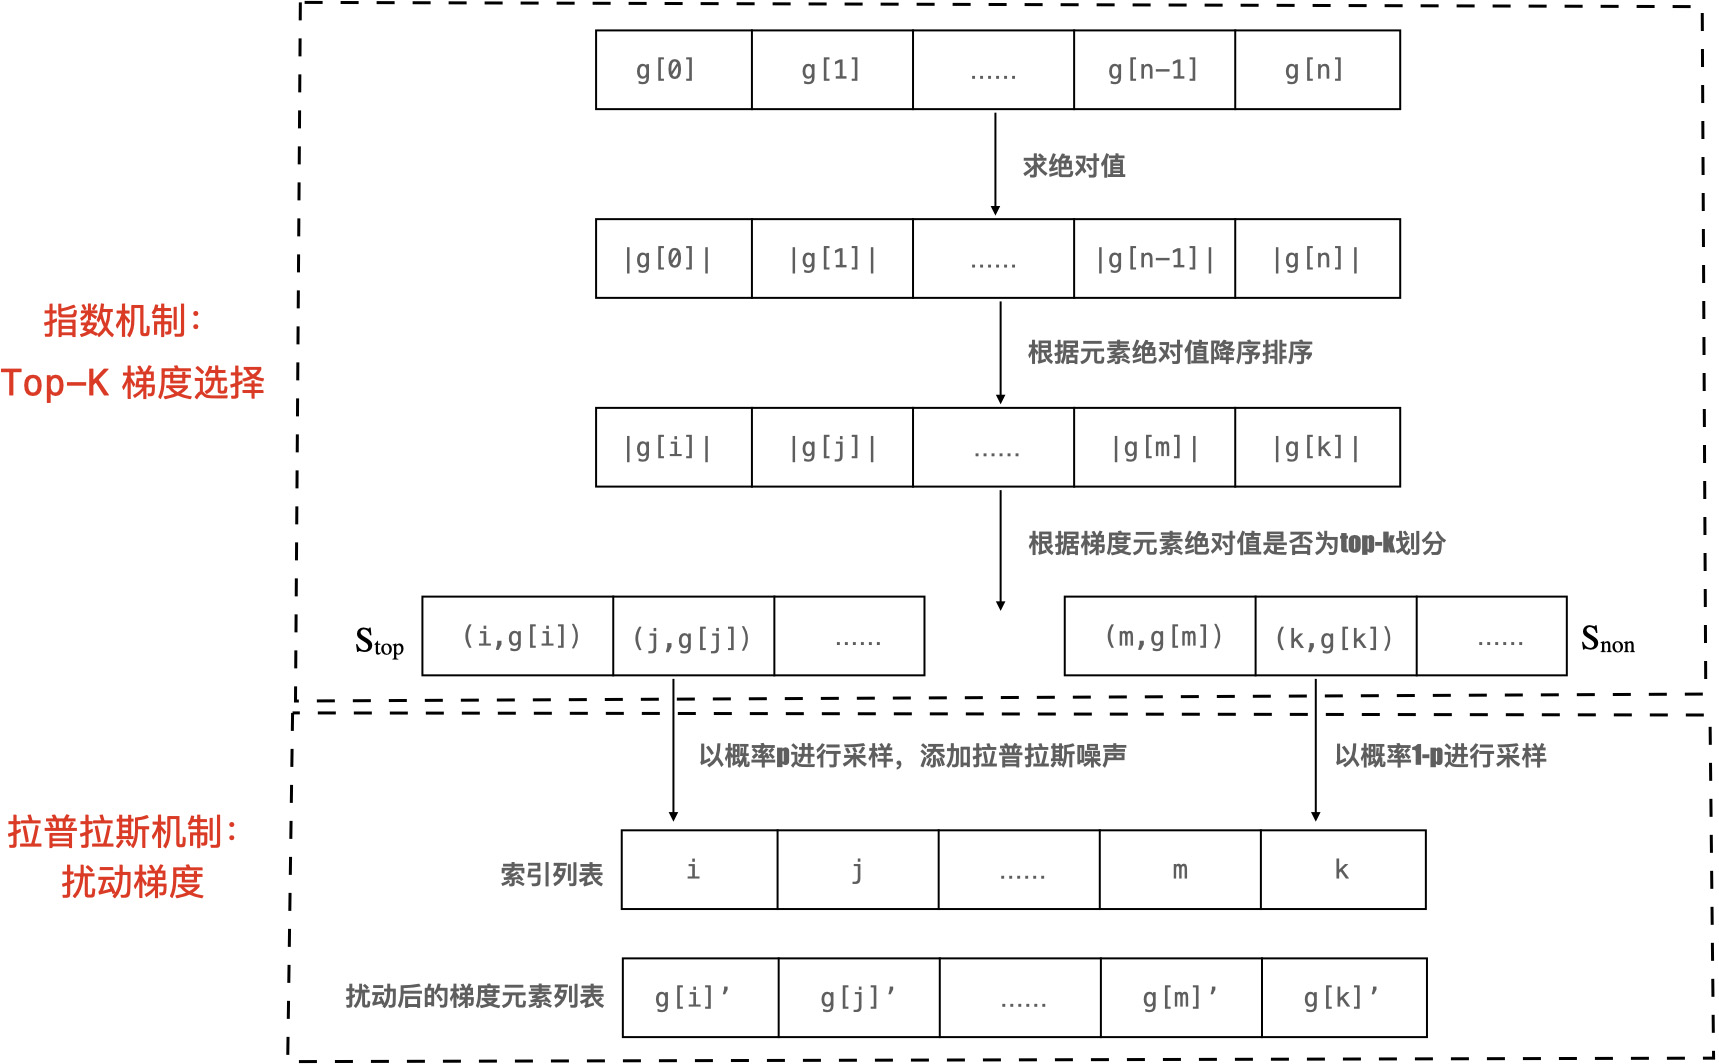
\includegraphics[scale=0.22]{fig2/C4/top-K流程图}%联邦学习的系统架构
	\caption{top-K梯度选择算法流程图}
	\label{fig:top-K梯度选择算法流程图}	
\end{figure}

首先构造一个二维数组,分别存储梯度值的索引$i$,梯度绝对值$\mathbf{g}[i]$。梯度的置信值$u_{i}$为1或者0,1表示该梯度值属于top-K,0反之。
对于第i个索引的梯度值$\mathbf{g}[i]$,我们将根据其索引对应的梯度置信值进行划分,得到top-K集合$S_{\text {top }} \leftarrow\left\{i \mid i \in \operatorname{Top}\left(\left|\tilde{x}_{i}\right|\right)\right\}$和非top-K集合$S_{\text {non-top}} \leftarrow\left\{i \mid i \in[n] \backslash S_{\text {top }}\right\}$。

\begin{figure}[!hbt]
\centering
	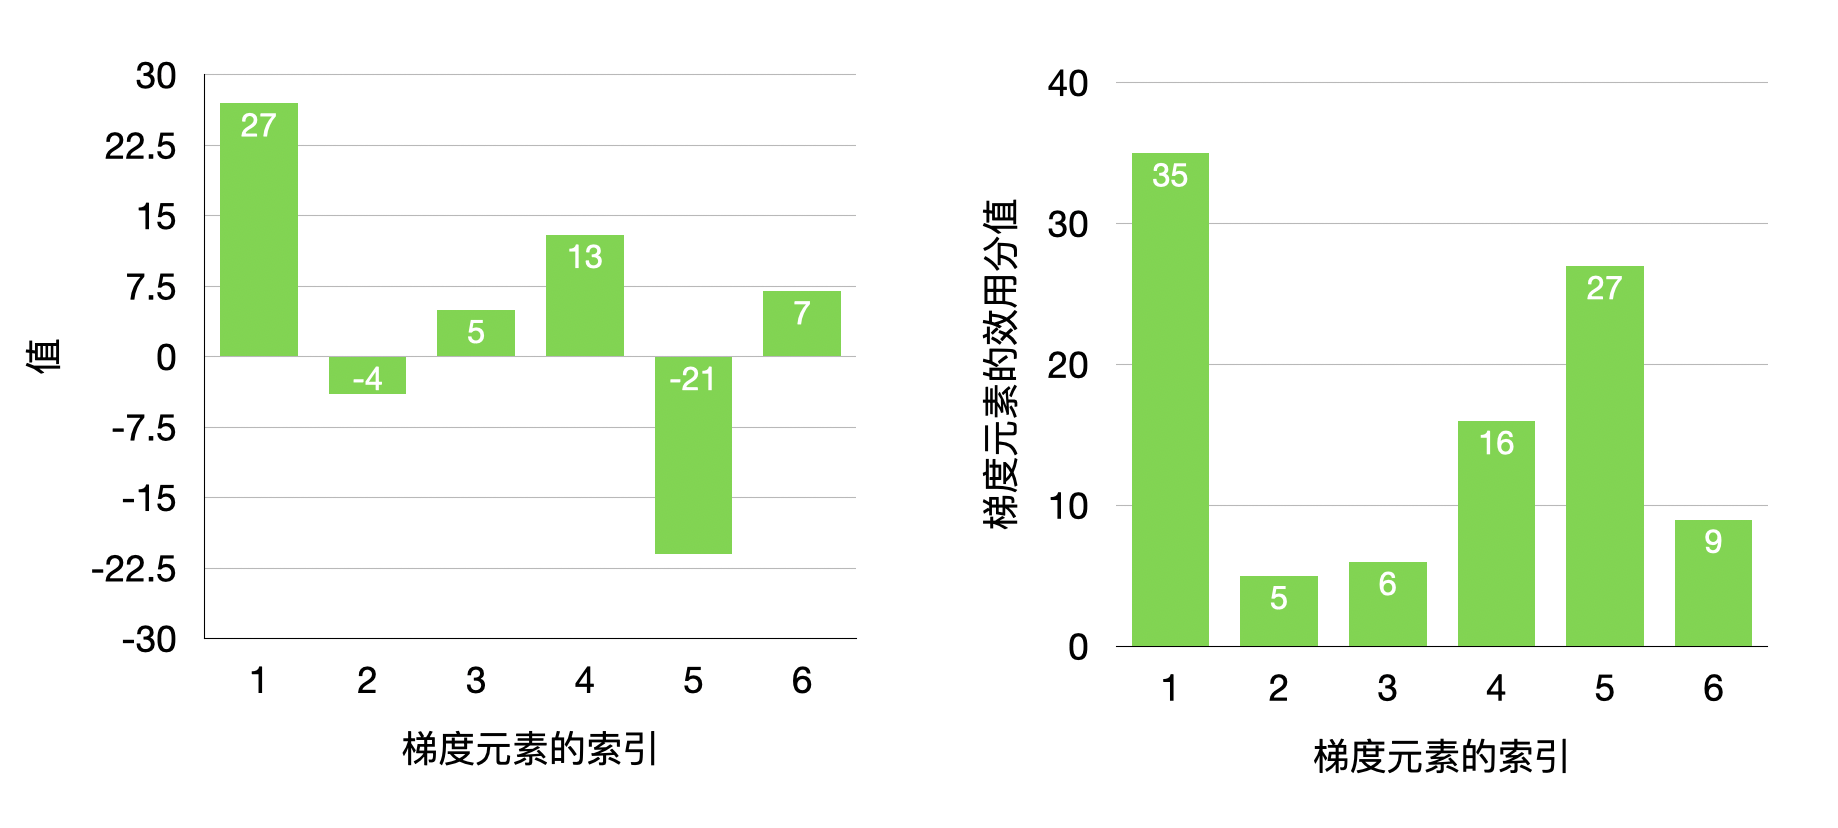
\includegraphics[scale=0.45]{fig2/C4/梯度值打分}%联邦学习的系统架构
	\caption{梯度元素的值及其效用评分}
	\label{fig:梯度元素的值及其效用评分}	
\end{figure}

如图\ref{fig:梯度元素的值及其效用评分}所示,当K=2时,根据梯度元素的绝对值进行降序排序,然后根据其索引对应的梯度值是否为top-K梯度值进行划分,得到,梯度置信向量$u=\left\{u_{1}, \cdots, u_{n}\right\}=\{1,0,0,0,1,0\}$,其中$S_{\text {top }}=\{1,5\}$,$S_{\text {non }}=\{2,3,4\}$。

接着对$S_{\text {top }}$和$S_{\text {non-top}} $集合按照不同的概率进行采样,从n个梯度绝对值及其索引构成的二维数组中以更高的概率p随机采样属于$S_{\text {top }}$的梯度值$\left\{g[1], \ldots, g[k]\right\} \in\{0,1\}^{k}$,在索引对应的梯度上直接添加拉普拉斯噪声:
$$
g[i]^{\prime}=g[i]+ \operatorname{Lap}\left(\frac{GS_{l}}{\epsilon_{i}}\right)
$$
以较低的概率1-p随机采样属于$S_{\text {non-top}} $的索引$\left\{g[1], \ldots, g[n-k+1]\right\} \in\{0,1\}^{n-k}$,将采样扰动后的新的梯度元素及其对应的索引分别存储到两个数组中,上传至混洗器。其中,$p=\frac{e^{\epsilon} \cdot k}{n-k+e^{\epsilon} \cdot k}$。这样的概率选择是满足$\epsilon$-差分隐私的,如下给出证明。

\begin{theorem}\label{隐私性证明-topk}
对于给定的梯度分值向量$u, u^{\prime}$,假设算法输出的索引为j,根据条件概率可以给出以下证明:
$$
\frac{\operatorname{Pr}[j \mid u]}{\operatorname{Pr}\left[j \mid u^{\prime}\right]} \leq \frac{\operatorname{Pr}\left[j \mid u_{j}=1\right]}{\operatorname{Pr}\left[j \mid u_{j}^{\prime}=0\right]}=\frac{p \frac{1}{k}}{(1-p) \frac{1}{n-k}}=e^{\epsilon}, \text { where } p=\frac{e^{\epsilon} k}{n-k+e^{\epsilon} \cdot k}.
$$
\end{theorem}

\begin{algorithm}[!htb]
	\caption{Top-K梯度选择算法}
	\label{Top-K梯度选择算法}
	\begin{algorithmic}[1]
		\footnotesize
		\STATE \textbf{输入:} 梯度向量$\mathbf{g}$,K,隐私预算$\epsilon$
		\STATE 初始化:tmp=[],TK=[],$S_{\text {top }}$=[],$S_{\text {non-top}}$=[] ∕∗tmp存储梯度绝对值,TK存储最终输出的梯度元素,$S_{\text {top }}$和$S_{\text {non-top}}$分别存储属于top-k元素的索引值和不属于top-k元素的索引值∗∕
		\FOR{ $\mathbf{g}[i] \in \mathbf{g}$}
			\STATE tmp.append({i,abs($\mathbf{g}[i]$)}); ∕∗tmp中的每个元素分别存储数组的索引和对应的元素绝对值∗∕
		\ENDFOR
		\STATE Sort tmp by tmp.values desc;∕∗根据梯度绝对值对tmp数组进行降序排序∗∕
		\FOR{tmp[i] in tmp}
				\IF{i <k } 
				\STATE $S_{\text {top }}$.append(i);
				\ELSE
				\STATE $S_{\text {non-top }}$.append(i);
				\ENDIF 
		\ENDFOR
		\FOR{each index $i \in S_{\text {top }} \cup S_{\text {non-top}}$}
				\IF{i in $S_{\text {top }}$}
				\STATE $y_{i, j}$=tmp[i].value+ $\operatorname{Lap}\left(\frac{GS_{l}}{\epsilon_{i}}\right)$;
				\ELSE
				\STATE $y_{i, j}$=${\omega_{\mathcal{R}}}_{tmp[i].value}$;
				\ENDIF
		\ENDFOR
		\STATE \textbf{输出:} $\left\langle index_{i}, y_{i}\right\rangle$
	\end{algorithmic}
\end{algorithm}

算法\ref{Top-K梯度选择算法}将满足$\epsilon_{1}-LDP$的梯度选择和满足$\epsilon_{2}-LDP$的拉普拉斯梯度扰动相结合,根据差分隐私的组合定理,整体算法满足$\left(\epsilon_{1}+\epsilon_{2}\right)-LDP$。
接着分析Top-K梯度选择算法的时间复杂度,与非隐私保护的SGD相比,LDP-SGD给本地设备带来了额外的计算成本。对于Top-K梯度选择算法,所有梯度元素的效用分数可以离线计算。对一个n维的向量进行排序需要消耗 $O(n \log n)$。计算n个维度的元素的效用分数需要消耗$O\left(n^{2}\right)$,元素取样需要消耗$O(n)$。因此,每个本地设备进行梯度选择和概率选择都需要额外的时间成本$O\left(n \log n+n^{2}+n\right)=O\left(n^{2}\right)$。Top-K梯度选择方案避免了每个维度的梯度扰动,计算成本相比于无梯度选择的LDP低很多。

\subsection{客户端动态采样}
原有的联邦学习是通过静态采样随机选择一部分客户参与联合平均。假使服务器最初设定的采样率为C,一旦有足够的客户更新达到初始采样率,服务器将停止接收更新,转而进行全局参数的聚合。在这个过程中,客户端的采样率保持不变,也就是所谓的静态采样,这种方法通过均匀地选择客户的数量来实现参数的聚合。

在深度学习的随机梯度下降算法中,学习率是影响神经网络训练的重要超参数之一,它控制着模型的学习速率,影响目标函数的收敛速度。学习率过大可能会使目标函数在最优值两侧来回移动;学习率过小可能会降低模型的收敛速度。如何设置最优的学习率参数是深度学习中的重要问题。现有经典的方案是在学习初期,设置较大的学习率,使网络以较快的速度进行梯度下降;而在训练后期,学习率逐渐递减,使得神经元的各个权重和偏置能更准确的接近最优解。动态调整学习率的方式包括指数衰减、自然指数衰减和多项式衰减等。本文基于神经网络中动态调整学习率的思想,在联邦学习中动态的调整客户端采样率,使用指数衰减率来递减训练过程中的采样率,其中子采样率R是当前通信回合t和衰减系数β的函数,如公式\ref{eq:动态子采样}所示:
\begin{equation}\label{eq:动态子采样}
R(t, \beta)=\frac{1}{\exp (\beta t)}
\end{equation}

算法\ref{客户端动态采样算法}是本文所设计的客户端动态采样算法,在每一轮的通信回合,用递减的采样速率乘以预设的初始采样率C,得到该轮的客户端采样率为$c=\frac{C}{\exp (\beta t)}$,采样率随着通信轮次的增加而减小。在训练初期,采样率更高,就有更多的客户参与到模型聚合中,加速联邦学习的收敛。一旦在初始训练的基础上得到出一个更通用的联邦学习模型,混洗器就会动态地减少参与全局聚合的客户端数量,以节省通信成本。即使在联邦学习训练刚开始时通信成本较高,但在几轮训练后,其选择的客户数量会迅速下降。整体来看,动态采样所运输的参数总量少于静态采样,其对全局模型的可用性的影响也较小,会在后续的实验部分给出证明。

\begin{algorithm}[!htb]
	\caption{客户端动态采样算法}
	\label{客户端动态采样算法}
	\begin{algorithmic}[1]
		\footnotesize
		\STATE \textbf{输入:} 初始客户端采样率:$C \in \mathbb{R}$,联邦学习协议设定的通信回合:$T \in \mathbb{N}^{+}$,参与联邦学习训练的本地设备集合: $S=\left\{s_{1}, \ldots, s_{M}\right\}$
		\FOR{ $t \in[T]$}
			\STATE 初始化空链表$L$,用于存放本轮通信回合参与聚合的本地设备上传的信息
			\STATE 计算客户端采样率:$c=\frac{C}{\exp (\beta t)}$
			\STATE 计算采样的客户端数量:$m=\max (c * M, 1)$
			\WHILE{len(L)<m}
				\STATE 向m个客户端发送连接请求
				\IF{第 i 个客户端返回ACK}
					\STATE 混洗器接收来自第i个客户端的加密信息$\Theta_{t}^{i}$
					\STATE $L$.add($\Theta_{t}^{i}$)
				\ENDIF
			\ENDWHILE
		\ENDFOR
	\end{algorithmic}
\end{algorithm}

\subsection{梯度混洗算法}
中央差分隐私基于可信第三方服务器的强依赖实现,本地差分隐私由于其在高维的联邦学习模型中,全局噪声的聚合导致统计结果的可用性降低。本文考虑在本地用户和中央服务器之间引入混洗器,用户在本地对数据添加随机扰动后,将加躁后的数据上传给混洗器,混洗器通过对加躁后的梯度向量进行shuffle,再将结果发送给中央服务器。梯度的混洗切断了梯度与客户端之间的关联关系,使中央服务器很难结合多个客户端的同步更新来推断任何本地设备的更多信息。通过在联邦学习中添加混洗器实现分布式的差分隐私,也叫做混洗差分隐私。混洗差分隐私兼顾了中央差分隐私下统计结果的准确性和本地差分隐私下数据安全水平高的优点。通过客户端的动态采样和梯度的混洗达到双重隐私放大效应,为实现相同的中央隐私保障所需的本地噪声更少,改善了隐私收益,缓解了高维数据聚合导致的模型可用性降低的问题。算法\ref{混洗器中的拆分混洗算法}是本文所设计的混洗器执行的拆分混洗算法。

\begin{algorithm}[!htb]
	\caption{混洗器中的拆分混洗算法}
	\label{混洗器中的拆分混洗算法}
	\begin{algorithmic}[1]
		\footnotesize
		\STATE \textbf{Input:} 本地客户端上传的索引列表和梯度元素列表$\left\langle index_{i,j}, y_{i,j}\right\rangle$
	    \FOR{$(index_{i,j}, y_{i,j}) \in \left\langle index_{i,j}, y_{i,j}\right\rangle$}
	    \STATE 对于$[n]$生成一个随机的排列组合$\pi^{(t)}$
	    \STATE $\pi(index_{i}) \leftarrow\left(index_{i_{1}},index_{i_{2}}, \ldots, index_{i_{n}}\right)$
	    \ENDFOR
	    \STATE 在时刻 $t_{i d}^{s}$将索引列表和梯度元素列表$\left\langle \pi(index_{i,j}), y_{i,j}\right\rangle$发送给中央服务器
	\end{algorithmic}
\end{algorithm}

如图\ref{fig:联邦学习安全混洗模型中执行参数拆分混洗的混洗器}所示,假使现有本地模型$X_{1}$,$X_{2}$,$X_{3}$,每个模型都有相同的结构,但权重值不同。原始的联邦学习框架是将本地训练后得到的参数直接发送到中央服务器,而本文中新增混洗器接受客户端上传的索引列表和梯度元素列表,在通信时刻(0,$T$),对于$[n]$生成一个随机的排列组合$\pi^{(t)}$,随机置换索引列表中元素的位置$\pi(index_{i}) \leftarrow\left(index_{i_{1}},index_{i_{2}}, \ldots, index_{i_{n}}\right)$,将索引列表和梯度元素列表$\left\langle index_{i,j}, y_{i,j}\right\rangle$发送给中央服务器。

在这个模型中,隐私性是针对整个用户数据集。每个本地用户的数据$x_{i}$都经过本地的二阶扰动和混洗器的混洗算法。根据差分隐私的串行组合定理,中央服务器接受到的经过本地扰动和混洗的数据:
$$
\left(\mathcal{S} \circ \text{top-K}^{M}\right)(\vec{x}):=\mathcal{S}\left(\text{top-K}\left(x_{1}\right), \ldots, \text{top-K}\left(x_{M}\right)\right)
$$
是满足$\left(\epsilon^{\prime}, \delta\right)$-差分隐私。其中$\epsilon^{\prime}=O\left(\frac{\epsilon \sqrt{\log (1 / \delta)}}{\sqrt{m}}\right)$。混洗结果并不会改变数据集的统计特性,也不会增加LDP的隐私预算。

\section{隐私性和收敛性证明}
\subsection{隐私性证明}
在算法\ref{联邦学习中的安全混洗算法}中,每个本地客户端采用Top-K梯度选择算法得到满足$\left(\epsilon_{1}+\epsilon_{2}\right)-LDP$的梯度元素列表和索引列表,将其上传至混洗器进行混洗后,所获取的数据满足 $\bar{\epsilon}-\mathrm{DP}$。从 $\left(\epsilon_{c}+\epsilon_{l}\right)$到 $\bar{\epsilon} $的转变可通过隐私放大理论证明,$\left(\epsilon_{c}+\epsilon_{l}\right)$对于较高的隐私预算,表示隐私保护的水平更低; $\bar{\epsilon}$对应于较低的隐私预算,表示隐私保护的水平更高。因此经过混洗器后,隐私性得到了增强,也就是所谓的隐私放大。隐私放大效应(Privacy Amplification)是针对客户端动态采样和梯度混洗算法增加隐私保护效用的理论分析。由差分隐私的强组合性可保证所有本地用用户采用Top-K梯度选择算法进行扰动后所得的数据总体都满足$\left(\epsilon_{c}+\epsilon_{l}\right)$-LDP,因此本节只需要分析客户端采样和混洗操作的隐私放大性,证明中央服务器接收到的数据满足$\bar{\epsilon}$-差分隐私。

% \begin{theorem}\label{隐私性证明}
% 算法\ref{联邦学习中的安全混洗算法}是满足$(\epsilon, \delta)-$差分隐私的,当对于任意$\delta$,$\delta>0$ ,并且有:
% $$
% \epsilon=\mathcal{O}\left(\epsilon_{0} \sqrt{\frac{q T \log (2 q T / \delta) \log (2 / \delta)}{n}}\right)
% $$
% \end{theorem}

假设在联邦学习模型中,初始设定的总通信回合为$[T]$。$\mathcal{M}_{t}\left(\theta_{t}, \mathcal{D}\right)$表示在第$t$轮通信回合对于数据集$\mathcal{D}$和模型参数为$\theta_{t}$部署混洗差分隐私机制,$\theta_{t+1}$表示模型的输出。因此,在数据集$\mathcal{D}=\bigcup_{i=1}^{m} \mathcal{D}_{i} \in \mathfrak{S}^{n}$上部署的混洗差分隐私机制定义如下:

\begin{equation}\label{eq:隐私性证明机制}
\mathcal{M}_{t}\left(\theta_{t} ; \mathcal{D}\right)=\mathcal{H}_{k n} \circ \mathcal{S}_{M,m}\left(\text{top-K}\left(\boldsymbol{x}_{i 1}^{t}\right), \ldots, \text{top-K}\left(\boldsymbol{x}_{i M}^{t}\right)\right)
\end{equation}

其中, $\mathcal{S}_{M, m}$表示从有M个元素的客户端集合中动态采样m个客户端的参数,$\text{top-K}\left(\boldsymbol{x}_{i 1}^{t}\right)$表示本地客户端采用Top-K梯度选择算法得到满足$\left(\epsilon_{1}+\epsilon_{2}\right)-LDP$的梯度向量。

% $\mathcal{G}_{i}=\operatorname{samp}_{r, s}\left(\text{top-K}\left(\boldsymbol{x}_{i 1}^{t}\right), \ldots, \text{top-K}\left(\boldsymbol{x}_{i r}^{t}\right)\right)$并且$\boldsymbol{x}_{i j}^{t}=$$\nabla_{\theta_{t}} f\left(\theta_{t} ; d_{i j}\right), \forall i \in[M], j \in[r]$。$\mathcal{H}_{k n}$表示在$kn$个数据样本上进行混洗操作

接下来我们给出$\mathcal{M}_{t}$的隐私性证明:

假设客户端$i \in[m]$的本地数据集为$\mathcal{D}_{i}=\left\{d_{i 1}, d_{i 2}, \ldots, d_{i r}\right\} \in \mathfrak{S}^{r}$,$\mathcal{D}=\bigcup_{i=1}^{m} \mathcal{D}_{i}$表示总体数据集。根据公式\ref{eq:隐私性证明机制},$\mathcal{Z}\left(\mathcal{D}^{(t)}\right)=\mathcal{H}_{k n}\left(\text{top-K}\left(\boldsymbol{x}_{1}^{t}\right), \ldots, \text{top-K}\left(\boldsymbol{x}_{k n}^{t}\right)\right)$表示对本地客户端进行模型训练,运行top-K梯度选择得到的$kn$个权重集合进行混洗。任取$\tilde{\delta}>0$,当$\left(\epsilon_{1}+\epsilon_{2}\right) \leq \frac{\log (kn / \log (1 / \tilde{\delta}))}{2}$时,算法$\mathcal{Z}$ 满足 $(\tilde{\epsilon}, \tilde{\delta})-\mathrm{DP}$差分隐私,可得:

\begin{equation}\label{eq:隐私性证明机制2}
\tilde{\epsilon}=\mathcal{O}\left(\min \left\{\left(\epsilon_{1}+\epsilon_{2}\right), 1\right\} e^{\left(\epsilon_{1}+\epsilon_{2}\right)} \sqrt{\frac{\log (1 / \tilde{\delta})}{k n}}\right)
\end{equation}

当$\left(\epsilon_{1}+\epsilon_{2}\right)=\mathcal{O}(1)$时,有$\tilde{\epsilon}=\mathcal{O}\left(\left(\epsilon_{1}+\epsilon_{2}\right) \sqrt{\frac{\log (1 / \tilde{\delta})}{k n}}\right)$。

如下给出证明:
令$\mathcal{T} \subseteq\{1, \ldots, m\}$表示在时刻$t$选取的m个客户端。对于$i \in \mathcal{T}$,$\mathcal{T}_{i} \subseteq\{1, \ldots, r\}$表示在时刻$t$客户端$i$所抽样的$s$条数据样本。对于任意的 $\mathcal{T} \in\left(\begin{array}{c}{[m]} \\ k\end{array}\right)$和$\mathcal{T}_{i} \in\left(\begin{array}{c}{[r]} \\ n\end{array}\right), i \in \mathcal{T}$,事先定义$\overline{\mathcal{T}}=\left(\mathcal{T}, \mathcal{T}_{i}, i \in \mathcal{T}\right)$, 对于 $i \in \mathcal{T}$有$\mathcal{D}^{\mathcal{T}_{i}}=\left\{d_{j}: j \in \mathcal{T}_{i}\right\}$,并且$\mathcal{D}^{\bar{\top}}=\left\{\mathcal{D}^{\mathcal{T}_{i}}: i \in \mathcal{T}\right\}$。$\mathcal{T}$和$\mathcal{T}_{i}, i \in \mathcal{T}$为抽样产生的任意子集,其中的随机性由客户端抽样和数据集抽样所决定。算法$\mathcal{M}_{t}$可以等价的表示为$\mathcal{M}_{t}=\mathcal{Z}\left(\mathcal{D}^{\overline{\mathcal{T}}}\right)$。

假设现有数据集:$\mathcal{D}^{\prime}=\left(\mathcal{D}_{1}^{\prime}\right) \bigcup\left(\cup_{i=2}^{m} \mathcal{D}_{i}\right) \in \mathfrak{S}^{n}$,其中数据集$\mathcal{D}_{1}^{\prime}=\left\{d_{11}^{\prime}, d_{12}, \ldots, d_{1 r}\right\}$和$\mathcal{D}_{1}=\left\{d_{11}, d_{12}, \ldots, d_{1 r}\right\}$为相邻数据集,它们的第$d_{11}$条和第$d_{11}^{\prime}$条数据样本不同。如果$\mathcal{M}_{t}$是满足$(\bar{\epsilon}, \bar{\delta})-\mathrm{DP}$差分隐私的,那么对于算法$\mathcal{M}_{t}$所选的任意子集$\mathcal{S}$ 都应该满足:
\begin{equation}\label{eq:隐私性证明3}
\operatorname{Pr}\left[\mathcal{M}_{t}(\mathcal{D}) \in \mathcal{S}\right] \leq e^{\bar{\epsilon}} \operatorname{Pr}\left[\mathcal{M}_{t}\left(\mathcal{D}^{\prime}\right) \in \mathcal{S}\right]+\bar{\delta}
\end{equation}

\begin{equation}\label{eq:隐私性证明4}
\operatorname{Pr}\left[\mathcal{M}_{t}\left(\mathcal{D}^{\prime}\right) \in \mathcal{S}\right] \leq e^{\bar{\epsilon}} \operatorname{Pr}\left[\mathcal{M}_{t}(\mathcal{D}) \in \mathcal{S}\right]+\bar{\delta}
\end{equation}

由于式\ref{eq:隐私性证明3}和\ref{eq:隐私性证明4}是对称的,因此只需要证明其中一条。将输出的概率分布分割成四个条件概率的总和,这取决于是否挑选了第一个客户端以及第一个客户端是否挑选了第一条数据记录的事件。

下文给出式\ref{eq:隐私性证明3}的证明:

令$q=\frac{k s}{m r}$,我们给出条件概率的定义:
\begin{equation}\label{eq:隐私性证明5}
\begin{array}{l}
A_{11}=\operatorname{Pr}\left[\mathcal{Z}\left(\mathcal{D}^{\overline{\mathcal{T}}}\right) \in \mathcal{S} \mid 1 \in \mathcal{T} \text { and } 1 \in \mathcal{T}_{1}\right] \\
A_{11}^{\prime}=\operatorname{Pr}\left[\mathcal{Z}\left(\mathcal{D}^{\prime} \overline{\mathcal{T}}\right) \in \mathcal{S} \mid 1 \in \mathcal{T} \text { and } 1 \in \mathcal{T}_{1}\right] \\
A_{10}=\operatorname{Pr}\left[\mathcal{Z}\left(\mathcal{D}^{\overline{\mathcal{T}}}\right) \in \mathcal{S} \mid 1 \in \mathcal{T} \text { and } 1 \notin \mathcal{T}_{1}\right]=\operatorname{Pr}\left[\mathcal{Z}\left(\mathcal{D}^{\prime \overline{\mathcal{T}}}\right) \in \mathcal{S} \mid 1 \in \mathcal{T} \text { and } 1 \notin \mathcal{T}_{1}\right] \\
A_{0}=\operatorname{Pr}\left[\mathcal{Z}\left(\mathcal{D}^{\bar{T}}\right) \in \mathcal{S} \mid 1 \notin \mathcal{T}\right]=\operatorname{Pr}\left[\mathcal{Z}\left(\mathcal{D}^{\prime \bar{\tau}}\right) \in \mathcal{S} \mid 1 \notin \mathcal{T}\right]
\end{array}
\end{equation}

令$q_{1}=\frac{k}{m}$,$q_{2}=\frac{s}{r}$,那么$q=q_{1} q_{2}$,然后可以得到:
\begin{equation}\label{eq:隐私性证明6}
\begin{aligned} 
\operatorname{Pr}\left[\mathcal{M}_{t}(\mathcal{D}) \in \mathcal{S}\right] &=q A_{11}+q_{1}\left(1-q_{2}\right) A_{10}+\left(1-q_{1}\right) A_{0}
\end{aligned}
\end{equation}

\begin{equation}\label{eq:隐私性证明7}
\begin{aligned} 
\operatorname{Pr}\left[\mathcal{M}_{t}\left(\mathcal{D}^{\prime}\right) \in \mathcal{S}\right] &=q A_{11}^{\prime}+q_{1}\left(1-q_{2}\right) A_{10}+\left(1-q_{1}\right) A_{0} 
\end{aligned}
\end{equation}

% 因此,我们可以得到:
% \begin{equation}\label{隐私性证明8}
% A_{11} \leq e^{\tilde{\epsilon}} A_{11}^{\prime}+\tilde{\delta}
% \end{equation}

% \begin{equation}\label{隐私性证明9}
% A_{11} \leq e^{\tilde{\epsilon}} A_{10}+\tilde{\delta}
% \end{equation}

% 如果$\mathcal{M}_{t}$是满足$(\bar{\epsilon}, \bar{\delta})-\mathrm{DP}$差分隐私的,则有:
% $$
% \operatorname{Pr}\left[\mathcal{Z}\left(\mathcal{D}^{\overline{\mathcal{T}}}\right) \in \mathcal{S} \mid \mathcal{T}, \mathcal{T}_{i}, i \in \mathcal{T}\right] \leq e^{\tilde{\epsilon}} \operatorname{Pr}\left[\mathcal{Z}\left(\mathcal{D}^{\overline{\mathcal{T}^{\prime}}}\right) \in \mathcal{S} \mid \mathcal{T}^{\prime}, \mathcal{T}_{i}^{\prime}, i \in \mathcal{T}^{\prime}\right]+\tilde{\delta}
% $$
{}
根据对称性,对式\ref{eq:隐私性证明6}进行证明:
\begin{equation}
\begin{aligned}
\operatorname{Pr} & {\left[\mathcal{M}_{t}(\mathcal{D}) \in \mathcal{S}\right]=q A_{11}+q_{1}\left(1-q_{2}\right) A_{10}+\left(1-q_{1}\right) A_{0} } \\
& \leq q\left(e^{\tilde{\epsilon}} \min \left\{A_{11}^{\prime}, A_{10}\right\}+\tilde{\delta}\right)+q_{1}\left(1-q_{2}\right) A_{10}+\left(1-q_{1}\right) A_{0} \\
&=q\left(\left(e^{\tilde{\epsilon}}-1\right) \min \left\{A_{11}^{\prime}, A_{10}\right\}+\min \left\{A_{11}^{\prime}, A_{10}\right\}\right)+q_{1}\left(1-q_{2}\right) A_{10}+\left(1-q_{1}\right) A_{0}+q \tilde{\delta} \\
&\left.\stackrel{(\text { a })}{\leq} q\left(e^{\tilde{\epsilon}}-1\right) \min \left\{A_{11}^{\prime}, A_{10}\right\}\right)+q A_{11}^{\prime}+q_{1}\left(1-q_{2}\right) A_{10}+\left(1-q_{1}\right) A_{0}+q \tilde{\delta} \\
& \stackrel{\text { (b) }}{\leq} q\left(\left(e^{\tilde{\epsilon}}-1\right)\left(q_{2} A_{11}^{\prime}+\left(1-q_{2}\right) A_{10}\right)\right)+\left(q A_{11}^{\prime}+q_{1}\left(1-q_{2}\right) A_{10}+\left(1-q_{1}\right) A_{0}\right)+q \tilde{\delta} \\
&=q_{2}\left(\left(e^{\tilde{\epsilon}}-1\right)\left(q_{1} q_{2} A_{11}^{\prime}+q_{1}\left(1-q_{2}\right) A_{10}\right)\right)+\left(q A_{11}^{\prime}+q_{1}\left(1-q_{2}\right) A_{10}+\left(1-q_{1}\right) A_{0}\right)+q \tilde{\delta} \\
&=\left(1+q_{2}\left(\left(e^{\tilde{\epsilon}}-1\right)\right)\left(q A_{11}^{\prime}+q_{1}\left(1-q_{2}\right) A_{10}\right)+\left(1-q_{1}\right) A_{0}\right)+q \tilde{\delta} \\
&=e^{\ln \left(1+q_{2}\left(e^{\tilde{\epsilon}}-1\right)\right)} \operatorname{Pr}\left[\mathcal{M}_{t}\left(\mathcal{D}^{\prime}\right) \in \mathcal{S}\right]+q \tilde{\delta}
\end{aligned}
\end{equation}

令$ks = qn$,可得top-K安全混洗算法满足$\bar{\epsilon}$-差分隐私的。

\subsection{模型收敛性分析}
在本节中,我们分析采用采样和混洗算法后模型的收敛性。

在算法\ref{联邦学习中的安全混洗算法}中,在每一轮迭代过程中,中央服务器聚合上传的$ks$个加躁后的梯度,如算法\ref{联邦学习中的安全混洗算法}的第22行所示,中央服务器进行聚合后得到结果:$\overline{\mathbf{g}}_{t} \leftarrow \frac{1}{k s} \sum_{i \in \mathcal{U}_{t}, j \in \mathcal{S}_{i t}} \left\langle y_{i,j} \right\rangle$,然后通过随机梯度下降算法更新全局模型参数:$\theta_{t+1} \leftarrow \prod_{\mathcal{C}}\left(\theta_{t}-\eta_{t} \overline{\mathbf{g}}_{t}\right)$。

既然随机扰动机制是无偏的,那么平均梯度$\overline{\mathbf{g}}_{t}$也是无偏的,也就是说,我们有 $\mathbb{E}\left[\overline{\mathbf{g}}_{t}\right]=\nabla_{\theta_{t}} F\left(\theta_{t}\right)$,其中期望是相对于客户端和数据点的随机抽样以及扰动机制的随机性而言的。

令$F(\theta)$为凸函数,考虑这样一个随机梯度下降算法:$\theta_{t+1} \leftarrow \prod_{\mathcal{C}}\left(\theta_{t}-\eta_{t} \mathbf{g}_{t}\right)$,$\mathbf{g}_{t}$满足$\mathbb{E}\left[\mathbf{g}_{t}\right]=\nabla_{\theta_{t}} F\left(\theta_{t}\right)$并且$\mathbb{E}\left\|\mathbf{g}_{t}\right\|_{2}^{2} \leq G^{2}$。当确定$\eta_{t}=\frac{D}{G \sqrt{t}}$,可以得到:
\begin{equation}\label{eq:模型收敛性证明1}
\mathbb{E}\left[F\left(\theta_{T}\right)\right]-F\left(\theta^{*}\right) \leq 2 D G \frac{2+\log (T)}{\sqrt{T}}=\mathcal{O}\left(D G \frac{\log (T)}{\sqrt{T}}\right)
\end{equation} 

由Nesterov等人在文献\upcite{ref50}中的证明可知,算法\ref{联邦学习中的安全混洗算法}的输出$\theta_{T}$满足:
\begin{equation}\label{eq:模型收敛性证明2}
\mathbb{E}\left[F\left(\theta_{T}\right)\right]-F\left(\theta^{*}\right) \leq \mathcal{O}\left(\frac{L D \log (T) \max \left\{d^{\frac{1}{2}-\frac{1}{p}}, 1\right\}}{\sqrt{T}}\left(1+\sqrt{\frac{c d}{q n}}\left(\frac{e^{\epsilon_{0}}+1}{e^{\epsilon_{0}}-1}\right)\right)\right)
\end{equation}

其中,存在$\sqrt{1+\frac{c d}{q n}\left(\frac{e^{\epsilon_{0}}+1}{e^{\epsilon_{0}}-1}\right)^{2}} \leq\left(1+\sqrt{\frac{c d}{q n}}\left(\frac{e^{\epsilon_{0}}+1}{e^{\epsilon_{0}-1}}\right)\right)$。

当$\sqrt{\frac{c d}{q n}}\left(\frac{e^{\epsilon_{0}}+1}{e^{\epsilon_{0}}-1}\right) \geq \Omega(1)$时,可以推导出:
\begin{equation}\label{eq:模型收敛性证明3}
\mathbb{E}\left[F\left(\theta_{T}\right)\right]-F\left(\theta^{*}\right) \leq \mathcal{O}\left(\frac{L D \log (T) \max \left\{d^{\frac{1}{2}-\frac{1}{p}}, 1\right\}}{\sqrt{T}} \sqrt{\frac{c d}{q n}}\left(\frac{e^{\epsilon_{0}}+1}{e^{\epsilon_{0}}-1}\right)\right)
\end{equation}

如果我们在算法\ref{联邦学习中的安全混洗算法}中设置学习率为$\eta_{t}=\frac{D}{G \sqrt{t}}$,其中\\$G^{2}=$ $L^{2} \max \left\{d^{1-\frac{2}{p}}, 1\right\}\left(1+\frac{c d}{q n}\left(\frac{e^{\epsilon_{0}}+1}{e^{\epsilon_{0}-1}}\right)^{2}\right)$。那么:

\begin{equation}\label{eq:模型收敛性证明4}
\mathbb{E}\left[F\left(\theta_{T}\right)\right]-F\left(\theta^{*}\right) \leq \\
\mathcal{O}\left(\frac{L D \log (T) \max \left\{d^{\frac{1}{2}-\frac{1}{p}}, 1\right\}}{\sqrt{T}} \sqrt{\frac{c d}{q n}}\left(\frac{e^{\epsilon_{0}}+1}{e^{\epsilon_{0}}-1}\right)\right)
\end{equation}

其中,当$p \in\{1, \infty\}$时,$c=4$否则$c=14$。

\begin{theorem}[随机梯度下降算法的收敛性]\label{随机梯度下降算法的收敛性}
假使有凸函数$F(\theta)$,数据集$D$的维度为$\mathcal{C}$,在模型训练过程中采用随机梯度下降算法$\theta_{t+1} \leftarrow \prod_{\mathcal{C}}\left(\theta_{t}-\eta_{t} \mathbf{g}_{t}\right)$,其中 $\mathbf{g}_{t}$满足$\mathbb{E}\left[\mathbf{g}_{t}\right]=\nabla_{\theta_{t}} F\left(\theta_{t}\right)$并且$\mathbb{E}\left\|\mathbf{g}_{t}\right\|_{2}^{2} \leq G^{2}$。当$\eta_{t}=$ $\frac{D}{G \sqrt{t}}$,$\mathbb{E}\left[F\left(\theta_{T}\right)\right]-F\left(\theta^{*}\right) \leq 2 D G\left(\frac{2+\log (T)}{\sqrt{T}}\right)$成立。
\end{theorem}

根据文献\upcite{ref50}中已有的标准随机梯度下降算法收敛结果中使用的定理\ref{随机梯度下降算法的收敛性}对$G^{2}$的约束条件,证明了安全混洗算法可在$G^{2}=$ $L^{2} \max \left\{d^{1-\frac{2}{p}}, 1\right\}\left(1+\frac{c d}{q n}\left(\frac{e^{\epsilon}+1}{e^{\epsilon-1}}\right)^{2}\right)$时达到全局最优解。

\section{实验评估}
\subsection{实验准备}
在本节中,我们进行实验来评估混洗器的性能。所有的实验都是用PYTHON语言编译的,其中每个用户都由配备6GB内存、四核2.36GHz Cortex A73处理器和四核Cortex A53 1.8GHz处理器的华为nova3安卓手机代替。中央服务器是用两台联想服务器模拟的,这两台服务器有2个英特尔(R)至强(R)E5-2620 2.10GHZ CPU,32GB内存,512SSD,2TB机械硬盘,运行于Ubuntu 18.04操作系统。

在实验过程中,我们选择了深度学习中常用的两个经典数据集--MNIST手写体数字识别数据集、FMNIST和CIFAR-10数据集进行实验,评估所提出的安全混洗框架。此外,我们让所有用户离线训练一个统一的卷积神经网络,以获得本地用户的梯度。在我们的实验中采用的模型网络结构为CNN,包括2个卷积层,两个池化层层和一个全连接层(32个神经元)。模型的激活函数为Softmax,并引入了DropOut正则以提高模型的泛化能力。下表展示了CNN的网络结构。

\begin{table}[H]
	\centering
	\begin{tabular}{cc}
		\hline
		神经层& 参数\\
		\hline
		卷积层& 8 × 8的16个滤波器,步长为2\\
		池化层& 2 × 2\\
		卷积层& 4 × 4的32个滤波器,步长为2\\
		池化层& 2 × 2\\
		全连接层& 32个神经元\\
		Softmax& 10个神经元\\
		\hline
	\end{tabular}
	\caption{安全混洗框架实验的模型网络结构}
	\label{tab1}
\end{table}

\subsection{实验设计}
在我们模拟的联邦学习环境中,我们设置本地客户端的总数为1000个,其中每个客户有一个本地数据集,每个客户都对梯度$\mathbf{g}_{t}\left(d_{i j}\right) \leftarrow \nabla_{\theta_{t}} f\left(\theta_{t} ; d_{i j}\right)$进行剪裁,梯度裁剪参数C=1/100。之后,运行Top-K梯度选择和拆分混洗算法,混洗器将参数上传至中央服务器进行安全聚合,更新全局参数。我们的算法运行了100个历时,在前80个历时中,我们将学习率设置为0.3,在剩余的历时中,将其降低到0.18。在每一次训练迭代过程中,本地客户端与混洗器、中央服务器进行交互计算得到安全聚合之后的全局梯度向量。我们设置了本地隐私参数$\sigma$=2,而中央隐私参数$\epsilon$的计算则是由我们来完成的。我们首先使用文献中\upcite{ref72}的定理5.3通过洗牌数值计算隐私放大率。然后,我们通过\ref{隐私性证明}中提出的子抽样计算隐私放大;最后,我们使用差分隐私的强组合性质来获得中央隐私参数$\epsilon$。

我们的实验主要分为两个部分:
\begin{enumerate}
\item [(1)] 在MNIST、FMNIST和CIFAR上评估安全混洗算法,评估参数:客户端数量$N$、梯度选择的比率、客户端采样比$f_{r}$和最大聚合次数对于模型分类准确率的影响。
\item [(2)] 将本文的安全混洗方案与基准方案(非隐私保护的联邦学习方案)、前人提出的隐私保护联邦学习方案(如表\ref{tab1}所示)进行对比,评估指标为模型分类准确率和通信性能。
\item [(3)] 在基于梯度选择和安全混洗的联邦学习模型上应用生成对抗网络攻击进行实验,评估模型的隐私保护效用。
\end{enumerate}

\begin{table}[H]
	\centering
	\begin{tabular}{cc}
		\hline
		基准方案名称& 具体算法\\
		\hline
		FL& 没有添加隐私保护机制的联邦学习模型\\
		PS-FL\upcite{ref67}& 通过选择性的参数更新实现隐私保护的分布式学习框架\\
		DP-FL& 基于中央差分隐私的联邦学习模型\\
		LDP-FL& 基于本地差分隐私的联邦学习模型\\
		KSA-FL& 本文的隐私保护方案,基于梯度选择和安全混洗的联邦学习模型\\
		\hline
	\end{tabular}
	\caption{安全混洗框架的比较方案}
	\label{tab1}
\end{table}

\subsection{结果分析}
\subsubsection{实验一(分析各个参数对模型准确率的影响)} 
在本文所设计的联邦学习安全混洗算法中,本地客户端的数量、梯度选择的比率、客户端采样比都是影响联邦学习模型分类准确率的因素。为了准确的反映每种参数对于准确率的影响,我们控制变量的进行实验。参考值如下:总客户端数量$N$为1000,梯度选择的比率分别为1\%、5\%、10\%、50\%、100\%,总通信回合为100,在前80个历时中,我们将学习率设置为0.3,在剩余的历时中,将其降低到0.18。隐私预算$\epsilon$分别为50、60、100。对于每一种参数组合进行模型训练,具体的实验结果如下文所示。

首先分析安全混洗模型中参与混洗的本地客户端数量对联邦模型分类精度的影响,如图\ref{fig:安全混洗模型中参与混洗的本地客户端数量对联合模型精度的影响}所示,通过Top-K梯度选择算法和拆分混洗算法,我们的安全混洗模型(下文简称KSA-FL)能够以较低的隐私成本实现较高的准确性。在训练中增加客户端数量N的同时,KSA-FL能达到的模型精度与不添加噪声的联邦学习几乎接近。与MNIST、FMNIST相比,CIFAR-10需要更多的客户端,这表明对于一个具有较大神经网络模型的更复杂的任务,当在更多的本地数据和更多的客户端上添加扰动之后,需要更多的通信回合才能使联邦学习模型达到更高的精度。

\begin{figure}[!hbt]
\centering
  	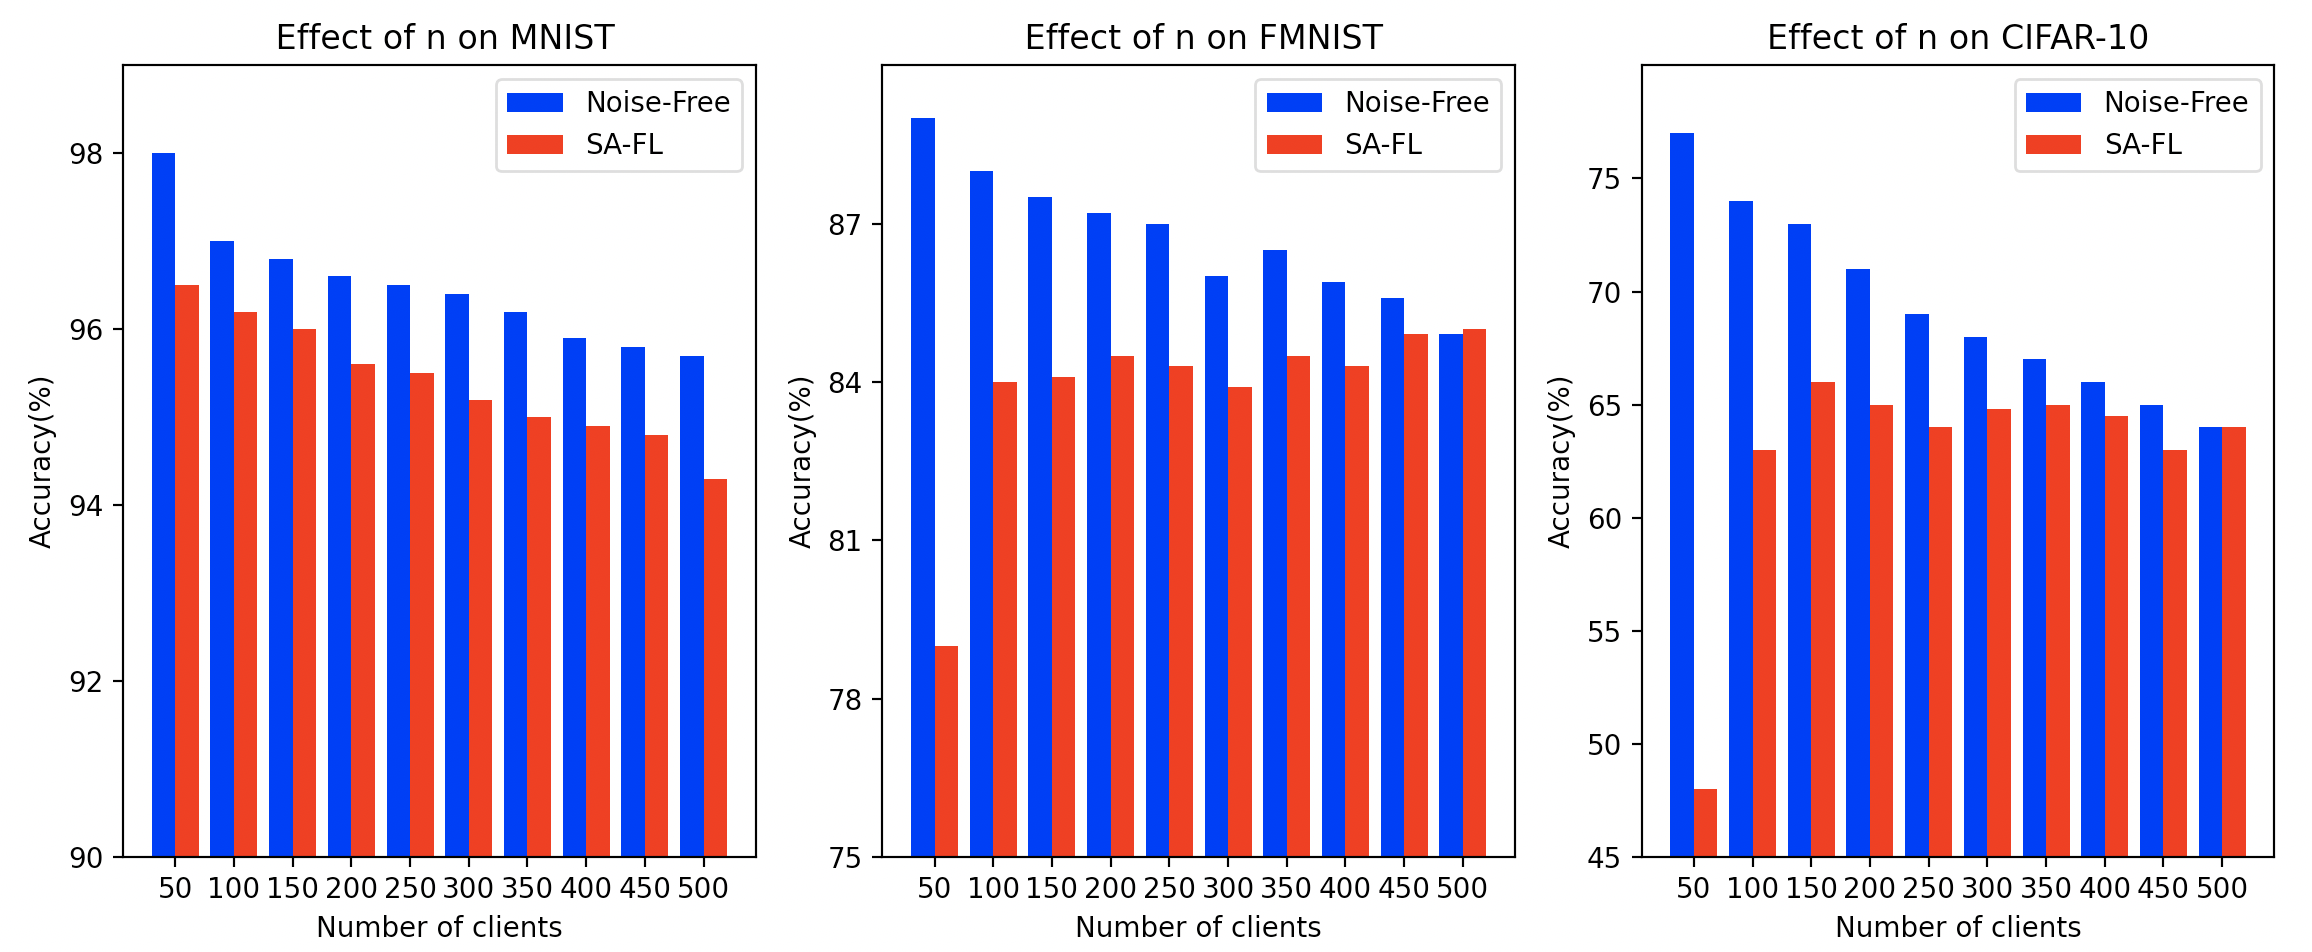
\includegraphics[scale=0.37]{fig2/C4/SA-FL1}%联邦学习的系统架构
	\caption{安全混洗模型中本地客户端数量对联邦学习模型训练精度的影响}
  	\label{fig:安全混洗模型中参与混洗的本地客户端数量对联合模型精度的影响} 
\end{figure}

如图\ref{fig:安全混洗模型中客户端采样比对联邦学习模型精度的影响}所示,当固定总客户端数量为100,在不同的隐私预算参数$\epsilon$=50、70、100和不添加隐私保护的联邦学习模型中,混洗器在每次迭代过程中随机采样部分客户端的梯度进行混洗。图\ref{fig:安全混洗模型中客户端采样比对联邦学习模型精度的影响}展示了全局损失函数值随客户端采样比的变化情况,总体来说,当客户端采样比为0.5左右时,损失函数值最小。联邦学习的隐私保护难点在于使用较低的隐私预算维持较高的模型精度,而选择适宜的客户端数量参与安全聚合会大大提升模型的收敛速度和通信性能。

\begin{figure}[!hbt]
\centering
  	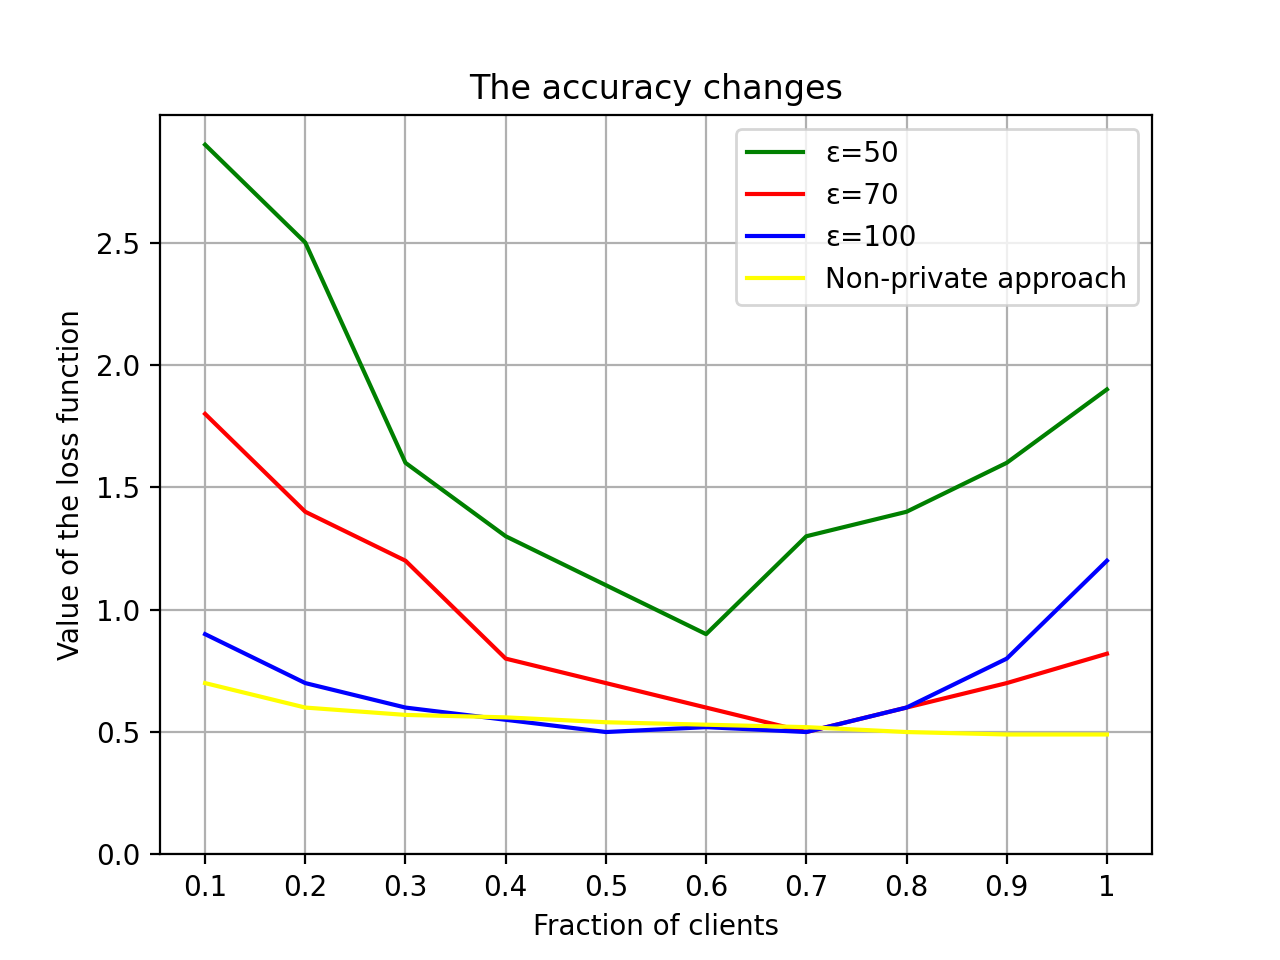
\includegraphics[scale=0.6]{fig2/C4/实验一客户端采样比}%联邦学习的系统架构
	\caption{安全混洗模型中客户端采样比对联邦学习模型训练精度的影响}
  	\label{fig:安全混洗模型中客户端采样比对联邦学习模型精度的影响} 
\end{figure}

\begin{figure}[!hbt]
\centering
  	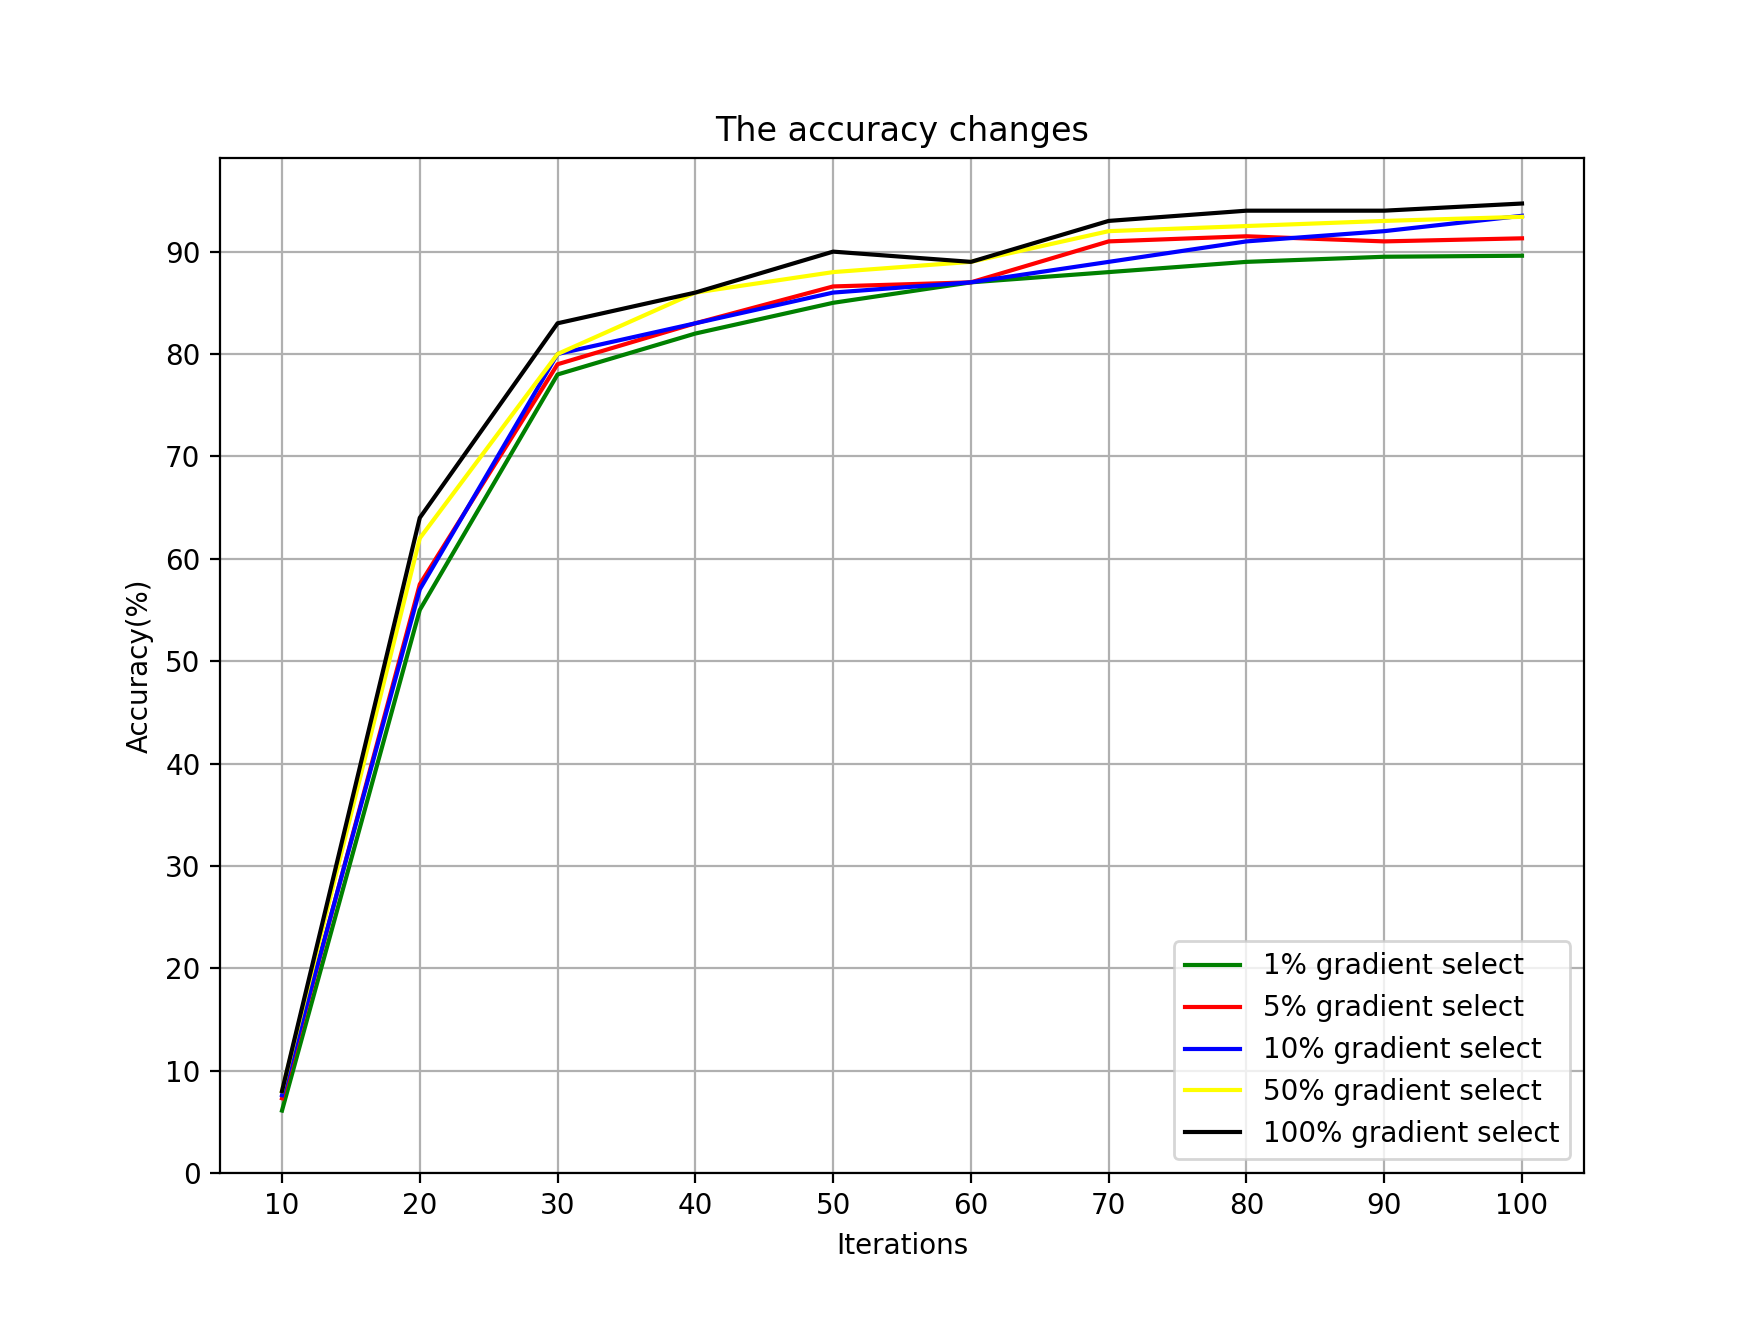
\includegraphics[scale=0.5]{fig2/C4/实验一K值}%联邦学习的系统架构
	\caption{安全混洗模型中梯度选择比率对联邦学习模型训练精度的影响}
  	\label{fig:安全混洗模型中梯度选择比率对联邦学习模型训练精度的影响} 
\end{figure}

如图\ref{fig:安全混洗模型中梯度选择比率对联邦学习模型训练精度的影响}展示了不同的梯度选择比率对联邦学习模型训练精度的影响,X轴表示联邦模型迭代次数。从图中的曲线变化情况可以看出,各个梯度选择比率的模型收敛速度接近,在70个训练回合后基本达到收敛,因此梯度选择并不会影响模型的收敛速度。1\%的梯度选择在历时100个训练回合后能达到83\%的准确率,100\%的梯度选择比率所能达到的模型准确率为95\%,相差了近10\%的准确率,可见部分梯度的丢弃确实丢失了部分的训练信息。当梯度选择比率低于10\%时,随着梯度选择比率的增加,模型的准确率也增加了接近3\%-5\%个百分点,然而当梯度选择比率为50\%时,模型在30个训练回合后的准确率基本与100\%的梯度选择比率所能达到的模型准确率接近。

在实验中,每一轮的迭代训练都需要由中央服务器和本地客户端交互计算,我们分别计算了不同的梯度选择比率在一次训练迭代中的通信开销,实验结果如表\ref{不同梯度选择比率的通信开销}所示。当梯度选择比率下降时,通信开销也基本呈比例下降。当Top-K梯度选择比率从100\%优化至50\%时,通信性能优化了大约1.99倍,而根据图\ref{fig:安全混洗模型中梯度选择比率对联邦学习模型训练精度的影响}所示,在梯度选择比率从100\%降低至50\%时,模型的训练准确率并不会受到太大影响,由此可见一定范围内的梯度选择可以较好的优化联邦学习模型的通信性能。

\begin{table}[H]
	\centering
	\begin{tabular}{cc}
		\hline
		Top-K/\%& 通信开销/KB\\
		\hline
		1& 167.022×2\\
		5& 863.317×2\\
		10& 1684.271×2\\
		50& 3502.151×2\\
		100& 6995.548×2\\
		\hline
	\end{tabular}
	\caption{不同梯度选择比率的通信开销}
	\label{不同梯度选择比率的通信开销}
\end{table}

\subsubsection{实验二(与前人的隐私保护方案进行对比实验)} 
我们将本文设计的基于梯度选择与安全混洗的联邦学习隐私保护方案(KSA-FL)的与FL、PS-FL、DP-FL、LDP-FL方案进行对比实验,选取的数据集为MNIST,网络模型为CNN5。我们比较了不同方案在给定相同的隐私预算($(0.2,5 \mathrm{e}-6)-\mathrm{DP}$)情况下,模型分类准确率变化情况。

\begin{figure}[!hbt]
\centering
  	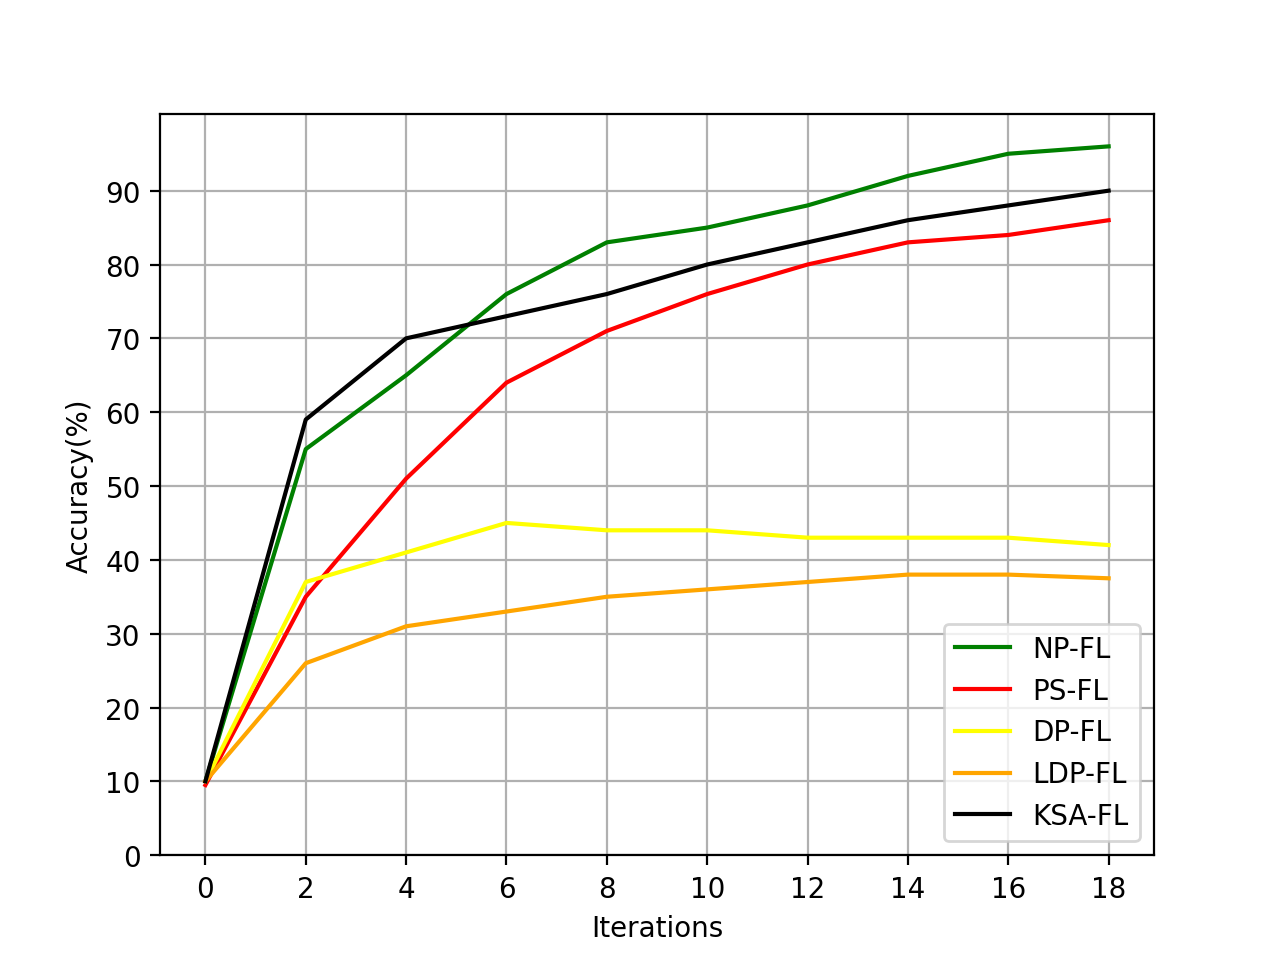
\includegraphics[scale=0.6]{fig2/C4/实验二}%联邦学习的系统架构
	\caption{不同隐私保护方案在MNIST数据集上训练的模型分类准确率变化情况}
  	\label{fig:不同隐私保护方案在MNIST数据集上训练的模型分类准确率变化情况} 
\end{figure}

在($(0.2,5 \mathrm{e}-6)-\mathrm{DP}$)的隐私预算下,无添加隐私保护的联邦学习基准模型在18个训练轮次后能达到94\%左右的准确率,其余四种实现了联邦学习隐私保护的方案中,本文所设计的Top-K安全混洗方案所能达到的准确率最高,在18个训练轮次后能达到90\%的准确率,而在训练开始阶段,模型的准确率提升速度甚至超过了无添加隐私保护的联邦学习基准模型,这表明Top-K梯度选择算法能有效的加速模型的学习速率。基于中央差分隐私的联邦学习隐私保护模型在18个训练轮次后能达到41\%左右的准确率,在6个训练轮次过后,模型就接近收敛。基于本地差分隐私的联邦学习隐私保护模型的分类准确率在这几种方案中的表现最低,正如上文分析的,本地差分隐私由于局部噪声带来的误差会随着维度系数的增加而加剧,从而大大降低模型的精度。

\subsubsection{实验三(针对攻击模型,分析该方案的隐私保护效用)} 
在第一章针对联邦学习的隐私威胁中,我们介绍了生成对抗网络攻击(GAN attack),GAN程序使一个鉴别性的深度学习网络与一个生成性的深度学习网络对立起来,形成对抗生成性深度学习网络,两者以零和博弈的思想进行对立训练。如图\ref{fig:联邦学习下的GAN模型}为联邦学习下GAN模型训练的示意图,生成器首先用随机噪声生成初始数据,然后在每个迭代中,它都被不断的训练,模仿被攻击者的训练集生成数据。鉴别器被训练来区分图像是来自原始数据库还是由GAN生成的。在联邦学习中,中央服务器通过聚合所有参与者上传的数据得到全局参数,而鉴别器参与了全局模型的训练,相当于在其他用户的训练数据上训练鉴别器,使得生成器有能力构造出与真实样本相似的伪样本。当生成器当鉴别器无法区分原始数据库的样本和生成器生成的样本时,模型的训练目标就完成了。

\begin{figure}[!hbt]
\centering
  	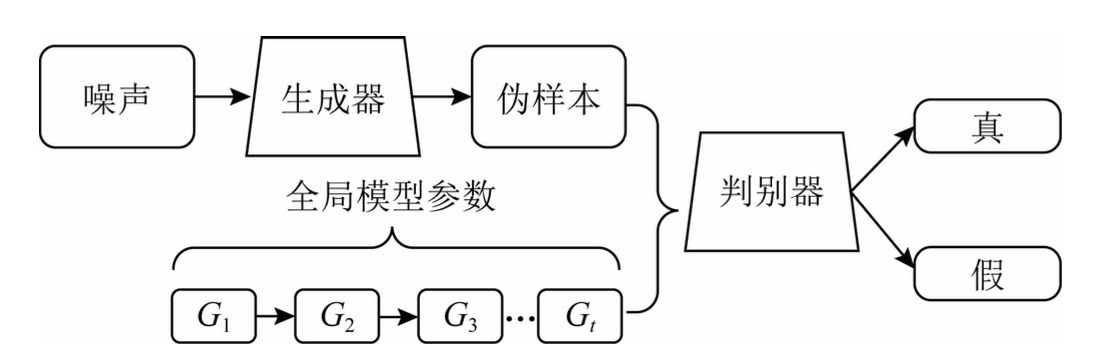
\includegraphics[scale=0.6]{fig2/C4/联邦学习GAN}%联邦学习的系统架构
	\caption{联邦学习下的GAN模型}
  	\label{fig:联邦学习下的GAN模型} 
\end{figure}

我们模拟的联邦学习环境中有十个本地客户端参与学习,数据集为MNIST。所有参与者都预先统一网络的训练架构和学习目标,这意味着他们就神经网络架构的类型和训练的标签达成一致。敌手A作为本地客户端参与联邦学习。为了模仿其他参与者的训练数据集的样本,我们在敌手一方采用GAN架构,其中GAN的鉴别器网络与联邦学习协议中的全局模型相同。当敌手在全局模型的准确率达到95\%后开始生成伪样本。被攻击的用户表示为V,V和A分别声明了标签[a,b]和[b,c]。敌手假装是深度学习协议的诚实参与者,但敌手会偷偷地影响学习过程,以欺骗V,使其释放关于目标类别的进一步细节。攻击者首先从中央服务器下载全局的训练参数,更新本地模型,同时在V不知情的情况下训练本地的对抗生成网络,生成fake类以模仿V的a类标签。当A的本地GAN模型中生成器当鉴别器无法区分原始数据库的样本和生成器生成的样本时,生成器生成的标签a即为最终数据。

\begin{figure}[!hbt]
\centering
  	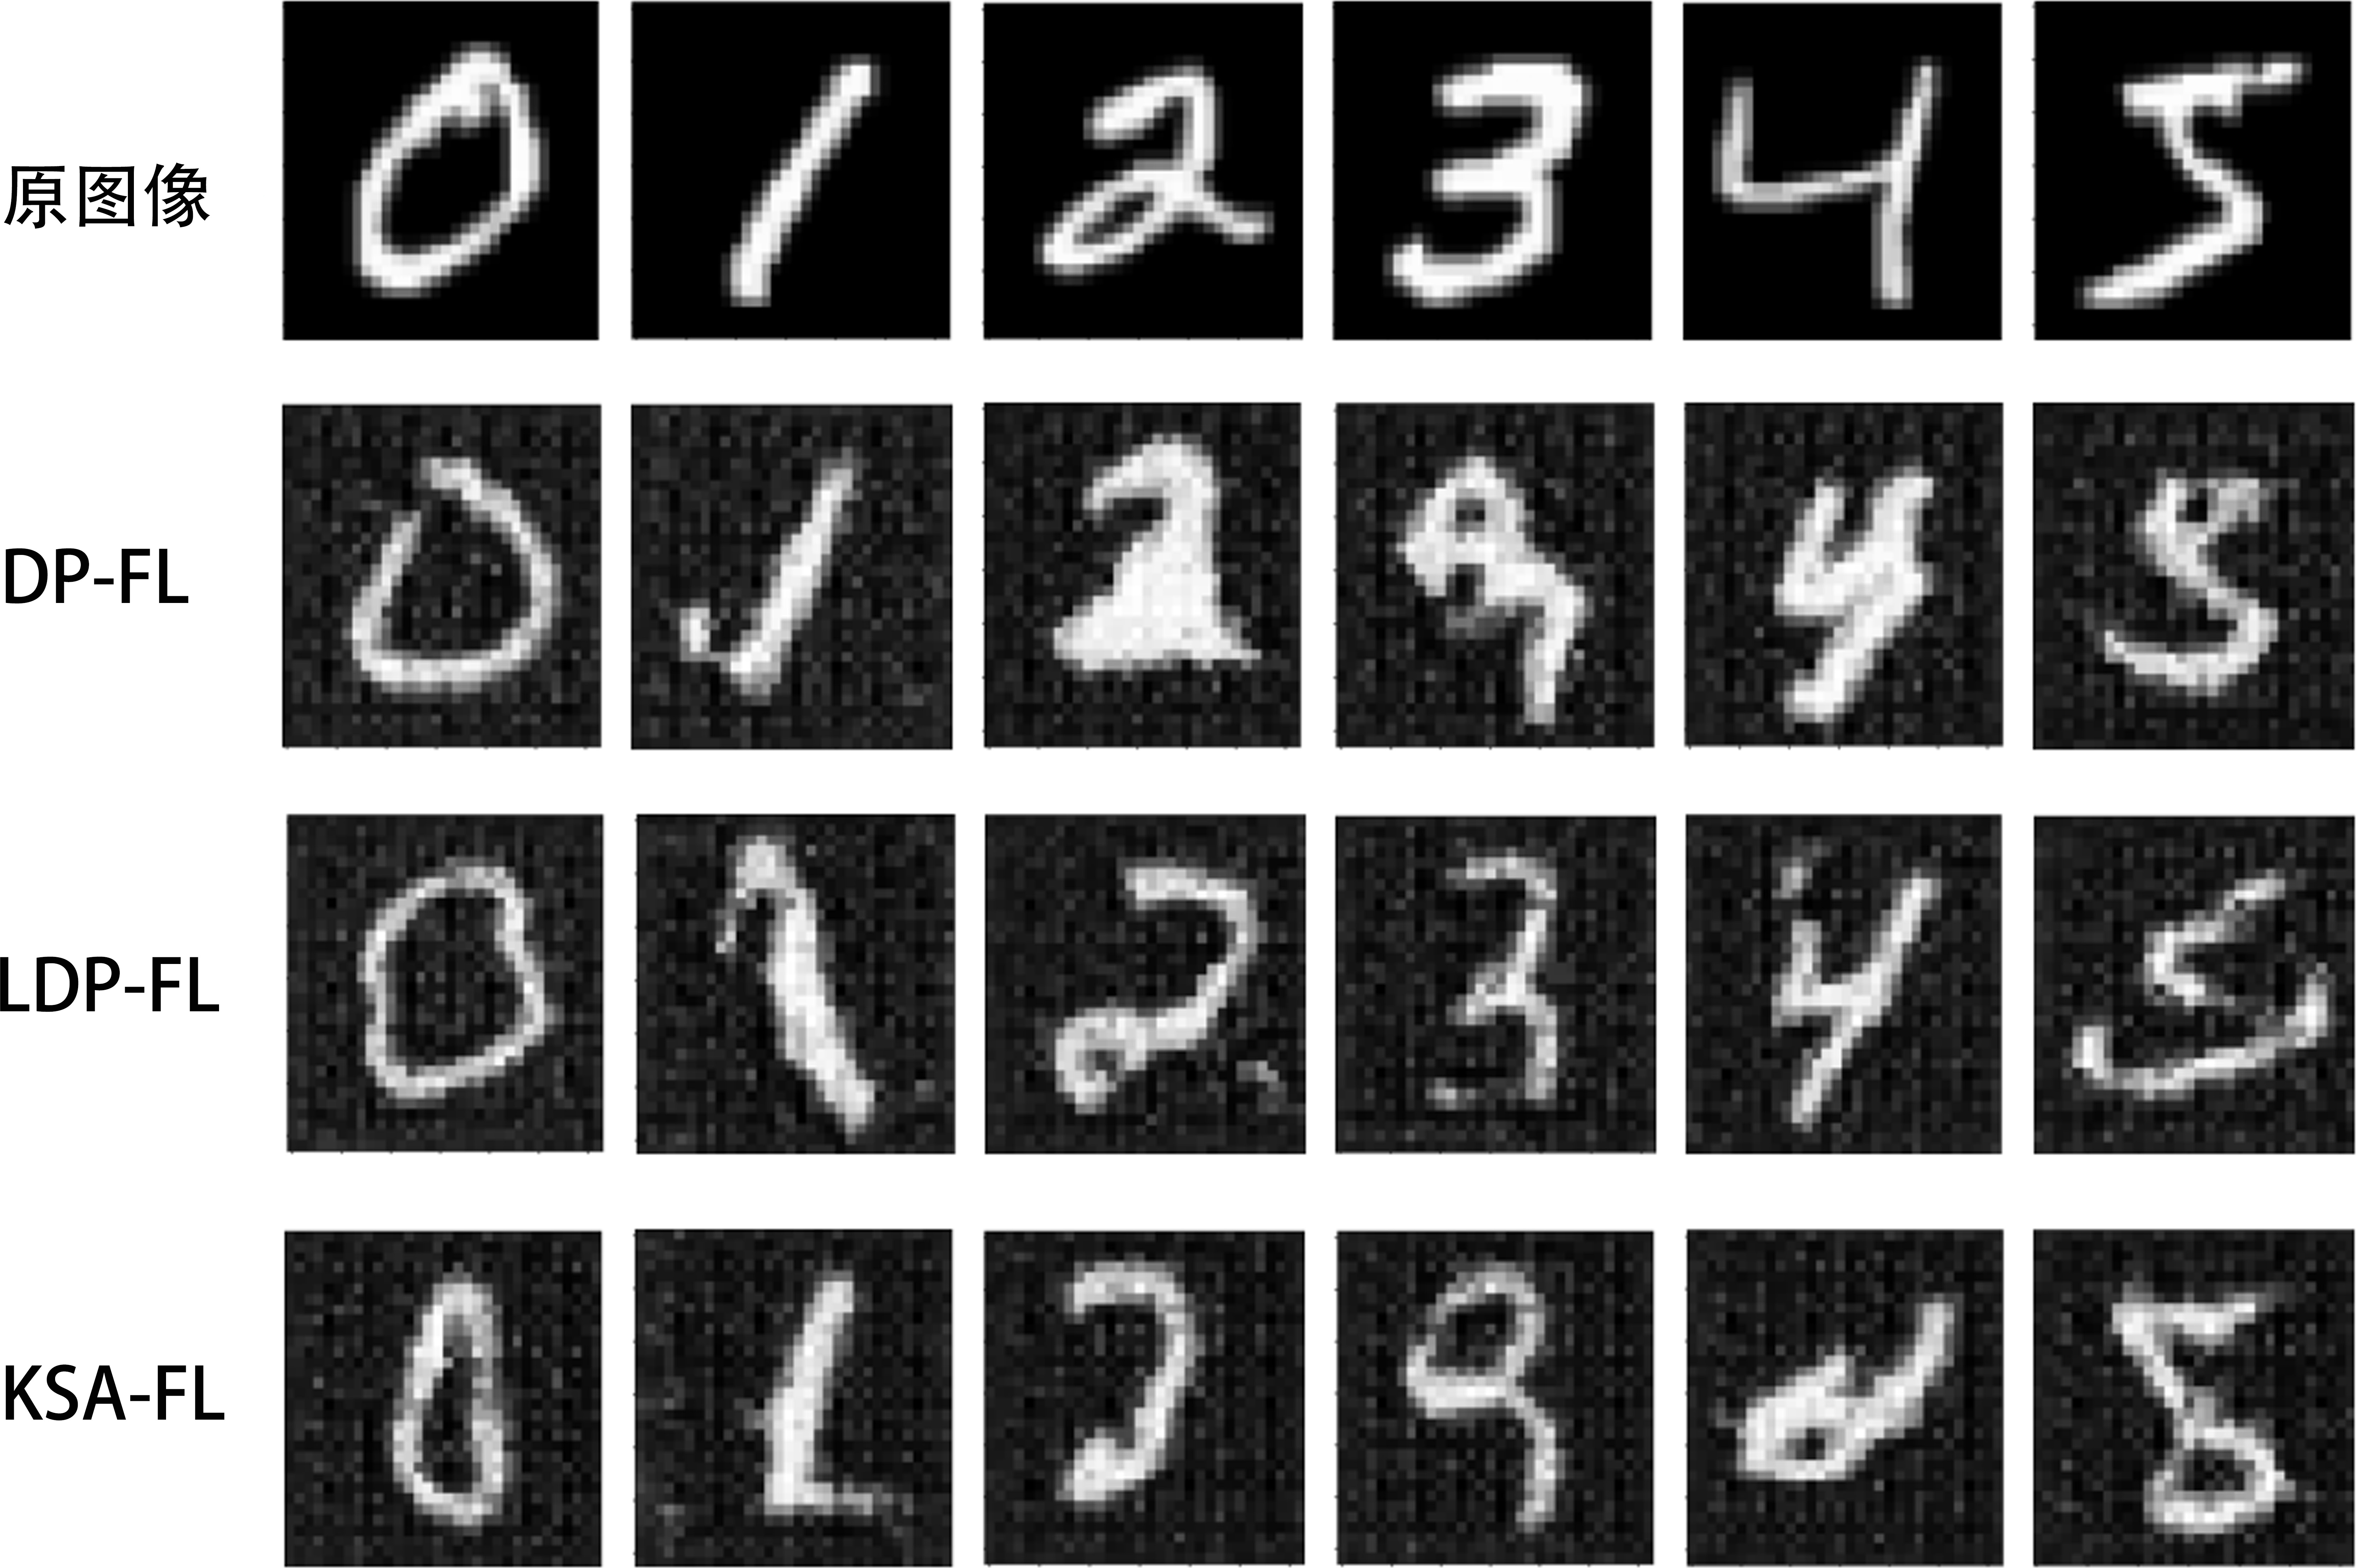
\includegraphics[scale=0.03]{fig2/C4/GAN攻击}%联邦学习的系统架构
	\caption{在MNIST数据集上对不同的隐私保护联邦学习算法下进行GAN攻击所生成的伪样本}
  	\label{fig:在MNIST数据集上对不同的隐私保护联邦学习算法下进行GAN攻击所生成的伪样本} 
\end{figure}

图\ref{fig:在MNIST数据集上对不同的隐私保护联邦学习算法下进行GAN攻击所生成的伪样本}显示了分别在不同的隐私保护联邦学习环境下进行GAN攻击,生成器训练的伪样本。第一行是其他参与者的真实训练样本。第二至四行分别是采用DP-FL、LDP-FL和KSA-FL隐私保护方案后攻击生成的伪样本。即使在联邦学习的本地模型或者全局模型上添加了差分隐私保护后,基于GAN的生成模型依然可以成功地模仿参与者的原始样本。但是这几种隐私保护的方案中,KSA-FL上所生成的伪样本相比DP-FL、LDP-FL与原始样本的差异更大,本节所设计的Top-K安全混洗方案(KSA-FL)在针对GAN攻击的隐私保护上效果更加显著。


\section{本章总结}
本章节我们针对联邦学习模型的整体框架进行了改进,基于稀疏向量和指数机制的思想,创造性地开发了Top-k 梯度选择算法,与拉普拉斯机制相结合,设计了满足$(\epsilon, \delta)$-本地差分隐私的算法。此外,我们将客户端采样和梯度混洗这两种隐私放大效应相结合,缓解了由维度系数增加而带来的隐私预算暴增和模型精度下降的问题。我们对方案进行了隐私性证明,表明此安全混洗算法可以保证$\varepsilon_{\mathrm{c}}$差分隐私,然后对此方案在中央服务器上的随机梯度下降算法进行了收敛性的分析,证明在凸函数上,梯度$\mathbf{g}_{t}$满足$\mathbb{E}\left[\mathbf{g}_{t}\right]=\nabla_{\theta_{t}} F\left(\theta_{t}\right)$时模型能达到全局收敛。最后,通过在三种基准数据集上进行实验,证明本章所设计的方案能提高全局模型的精度,也保证在更低的隐私成本下达到相同的隐私预算,且降低了通信成本。



